\documentclass[1p]{elsarticle_modified}
%\bibliographystyle{elsarticle-num}

%\usepackage[colorlinks]{hyperref}
%\usepackage{abbrmath_seonhwa} %\Abb, \Ascr, \Acal ,\Abf, \Afrak
\usepackage{amsfonts}
\usepackage{amssymb}
\usepackage{amsmath}
\usepackage{amsthm}
\usepackage{scalefnt}
\usepackage{amsbsy}
\usepackage{kotex}
\usepackage{caption}
\usepackage{subfig}
\usepackage{color}
\usepackage{graphicx}
\usepackage{xcolor} %% white, black, red, green, blue, cyan, magenta, yellow
\usepackage{float}
\usepackage{setspace}
\usepackage{hyperref}

\usepackage{tikz}
\usetikzlibrary{arrows}

\usepackage{multirow}
\usepackage{array} % fixed length table
\usepackage{hhline}

%%%%%%%%%%%%%%%%%%%%%
\makeatletter
\renewcommand*\env@matrix[1][\arraystretch]{%
	\edef\arraystretch{#1}%
	\hskip -\arraycolsep
	\let\@ifnextchar\new@ifnextchar
	\array{*\c@MaxMatrixCols c}}
\makeatother %https://tex.stackexchange.com/questions/14071/how-can-i-increase-the-line-spacing-in-a-matrix
%%%%%%%%%%%%%%%

\usepackage[normalem]{ulem}

\newcommand{\msout}[1]{\ifmmode\text{\sout{\ensuremath{#1}}}\else\sout{#1}\fi}
%SOURCE: \msout is \stkout macro in https://tex.stackexchange.com/questions/20609/strikeout-in-math-mode

\newcommand{\cancel}[1]{
	\ifmmode
	{\color{red}\msout{#1}}
	\else
	{\color{red}\sout{#1}}
	\fi
}

\newcommand{\add}[1]{
	{\color{blue}\uwave{#1}}
}

\newcommand{\replace}[2]{
	\ifmmode
	{\color{red}\msout{#1}}{\color{blue}\uwave{#2}}
	\else
	{\color{red}\sout{#1}}{\color{blue}\uwave{#2}}
	\fi
}

\newcommand{\Sol}{\mathcal{S}} %segment
\newcommand{\D}{D} %diagram
\newcommand{\A}{\mathcal{A}} %arc


%%%%%%%%%%%%%%%%%%%%%%%%%%%%%5 test

\def\sl{\operatorname{\textup{SL}}(2,\Cbb)}
\def\psl{\operatorname{\textup{PSL}}(2,\Cbb)}
\def\quan{\mkern 1mu \triangleright \mkern 1mu}

\theoremstyle{definition}
\newtheorem{thm}{Theorem}[section]
\newtheorem{prop}[thm]{Proposition}
\newtheorem{lem}[thm]{Lemma}
\newtheorem{ques}[thm]{Question}
\newtheorem{cor}[thm]{Corollary}
\newtheorem{defn}[thm]{Definition}
\newtheorem{exam}[thm]{Example}
\newtheorem{rmk}[thm]{Remark}
\newtheorem{alg}[thm]{Algorithm}

\newcommand{\I}{\sqrt{-1}}
\begin{document}

%\begin{frontmatter}
%
%\title{Boundary parabolic representations of knots up to 8 crossings}
%
%%% Group authors per affiliation:
%\author{Yunhi Cho} 
%\address{Department of Mathematics, University of Seoul, Seoul, Korea}
%\ead{yhcho@uos.ac.kr}
%
%
%\author{Seonhwa Kim} %\fnref{s_kim}}
%\address{Center for Geometry and Physics, Institute for Basic Science, Pohang, 37673, Korea}
%\ead{ryeona17@ibs.re.kr}
%
%\author{Hyuk Kim}
%\address{Department of Mathematical Sciences, Seoul National University, Seoul 08826, Korea}
%\ead{hyukkim@snu.ac.kr}
%
%\author{Seokbeom Yoon}
%\address{Department of Mathematical Sciences, Seoul National University, Seoul, 08826,  Korea}
%\ead{sbyoon15@snu.ac.kr}
%
%\begin{abstract}
%We find all boundary parabolic representation of knots up to 8 crossings.
%
%\end{abstract}
%\begin{keyword}
%    \MSC[2010] 57M25 
%\end{keyword}
%
%\end{frontmatter}

%\linenumbers
%\tableofcontents
%
\newcommand\colored[1]{\textcolor{white}{\rule[-0.35ex]{0.8em}{1.4ex}}\kern-0.8em\color{red} #1}%
%\newcommand\colored[1]{\textcolor{white}{ #1}\kern-2.17ex	\textcolor{white}{ #1}\kern-1.81ex	\textcolor{white}{ #1}\kern-2.15ex\color{red}#1	}

{\Large $\underline{12a_{0867}~(K12a_{0867})}$}

\setlength{\tabcolsep}{10pt}
\renewcommand{\arraystretch}{1.6}
\vspace{1cm}\begin{tabular}{m{100pt}>{\centering\arraybackslash}m{274pt}}
\multirow{5}{120pt}{
	\centering
	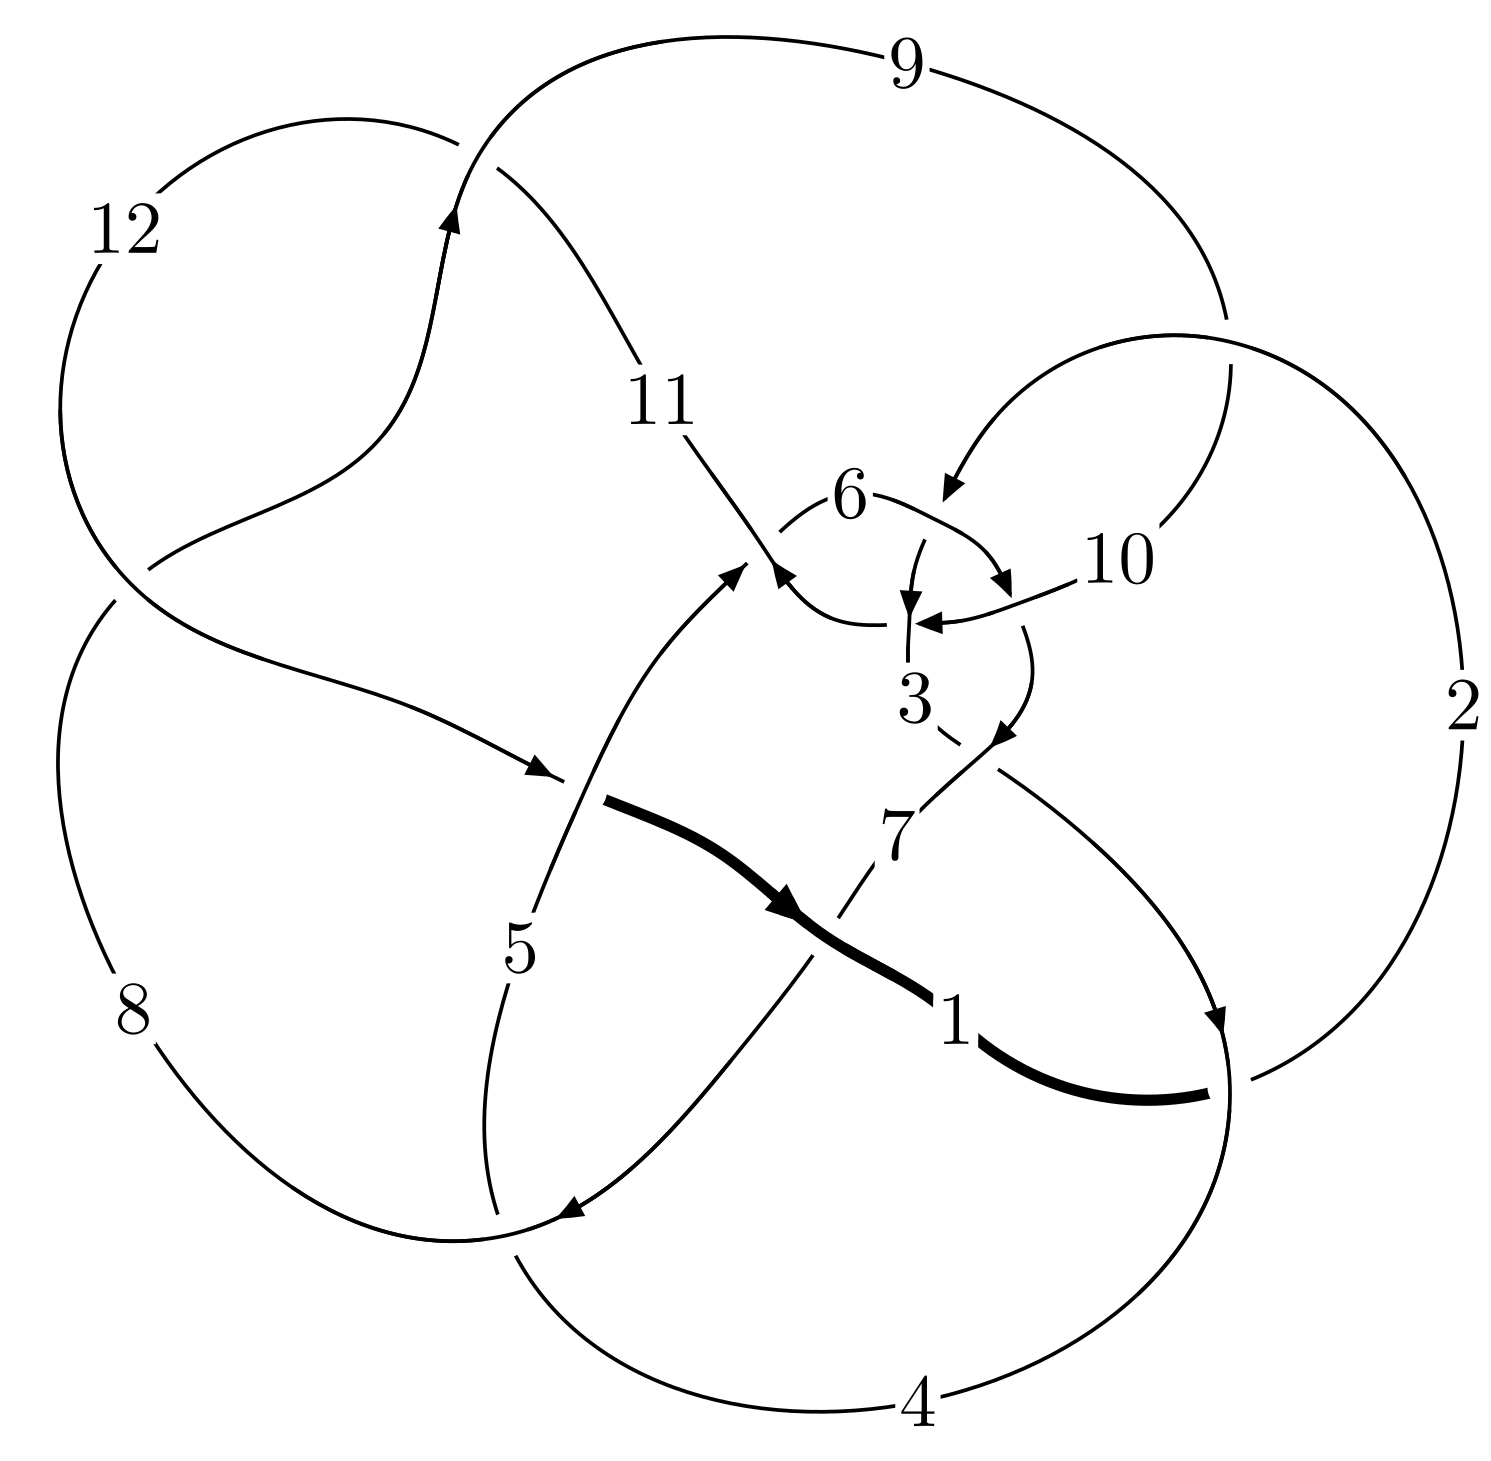
\includegraphics[width=112pt]{../../../GIT/diagram.site/Diagrams/png/1668_12a_0867.png}\\
\ \ \ A knot diagram\footnotemark}&
\allowdisplaybreaks
\textbf{Linearized knot diagam} \\
\cline{2-2}
 &
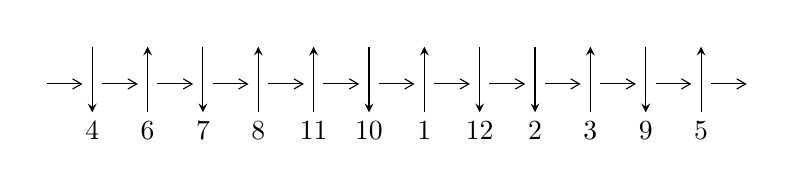
\begin{tikzpicture}[x=20pt, y=17pt]
	% nodes
	\node (C0) at (0, 0) {};
	\node (C1) at (1, 0) {};
	\node (C1U) at (1, +1) {};
	\node (C1D) at (1, -1) {4};

	\node (C2) at (2, 0) {};
	\node (C2U) at (2, +1) {};
	\node (C2D) at (2, -1) {6};

	\node (C3) at (3, 0) {};
	\node (C3U) at (3, +1) {};
	\node (C3D) at (3, -1) {7};

	\node (C4) at (4, 0) {};
	\node (C4U) at (4, +1) {};
	\node (C4D) at (4, -1) {8};

	\node (C5) at (5, 0) {};
	\node (C5U) at (5, +1) {};
	\node (C5D) at (5, -1) {11};

	\node (C6) at (6, 0) {};
	\node (C6U) at (6, +1) {};
	\node (C6D) at (6, -1) {10};

	\node (C7) at (7, 0) {};
	\node (C7U) at (7, +1) {};
	\node (C7D) at (7, -1) {1};

	\node (C8) at (8, 0) {};
	\node (C8U) at (8, +1) {};
	\node (C8D) at (8, -1) {12};

	\node (C9) at (9, 0) {};
	\node (C9U) at (9, +1) {};
	\node (C9D) at (9, -1) {2};

	\node (C10) at (10, 0) {};
	\node (C10U) at (10, +1) {};
	\node (C10D) at (10, -1) {3};

	\node (C11) at (11, 0) {};
	\node (C11U) at (11, +1) {};
	\node (C11D) at (11, -1) {9};

	\node (C12) at (12, 0) {};
	\node (C12U) at (12, +1) {};
	\node (C12D) at (12, -1) {5};
	\node (C13) at (13, 0) {};

	% arrows
	\draw[->,>={angle 60}]
	(C0) edge (C1) (C1) edge (C2) (C2) edge (C3) (C3) edge (C4) (C4) edge (C5) (C5) edge (C6) (C6) edge (C7) (C7) edge (C8) (C8) edge (C9) (C9) edge (C10) (C10) edge (C11) (C11) edge (C12) (C12) edge (C13) ;	\draw[->,>=stealth]
	(C1U) edge (C1D) (C2D) edge (C2U) (C3U) edge (C3D) (C4D) edge (C4U) (C5D) edge (C5U) (C6U) edge (C6D) (C7D) edge (C7U) (C8U) edge (C8D) (C9U) edge (C9D) (C10D) edge (C10U) (C11U) edge (C11D) (C12D) edge (C12U) ;
	\end{tikzpicture} \\
\hhline{~~} \\& 
\textbf{Solving Sequence} \\ \cline{2-2} 
 &
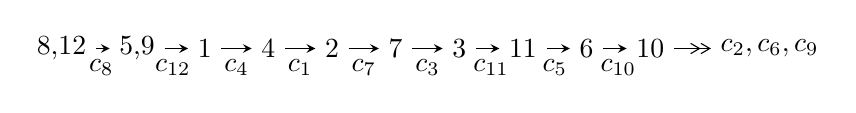
\begin{tikzpicture}[x=23pt, y=7pt]
	% node
	\node (A0) at (-1/8, 0) {8,12};
	\node (A1) at (17/16, 0) {5,9};
	\node (A2) at (17/8, 0) {1};
	\node (A3) at (25/8, 0) {4};
	\node (A4) at (33/8, 0) {2};
	\node (A5) at (41/8, 0) {7};
	\node (A6) at (49/8, 0) {3};
	\node (A7) at (57/8, 0) {11};
	\node (A8) at (65/8, 0) {6};
	\node (A9) at (73/8, 0) {10};
	\node (C1) at (1/2, -1) {$c_{8}$};
	\node (C2) at (13/8, -1) {$c_{12}$};
	\node (C3) at (21/8, -1) {$c_{4}$};
	\node (C4) at (29/8, -1) {$c_{1}$};
	\node (C5) at (37/8, -1) {$c_{7}$};
	\node (C6) at (45/8, -1) {$c_{3}$};
	\node (C7) at (53/8, -1) {$c_{11}$};
	\node (C8) at (61/8, -1) {$c_{5}$};
	\node (C9) at (69/8, -1) {$c_{10}$};
	\node (A10) at (11, 0) {$c_{2},c_{6},c_{9}$};

	% edge
	\draw[->,>=stealth]	
	(A0) edge (A1) (A1) edge (A2) (A2) edge (A3) (A3) edge (A4) (A4) edge (A5) (A5) edge (A6) (A6) edge (A7) (A7) edge (A8) (A8) edge (A9) ;
	\draw[->>,>={angle 60}]	
	(A9) edge (A10);
\end{tikzpicture} \\ 

\end{tabular} \\

\footnotetext{
The image of knot diagram is generated by the software ``\textbf{Draw programme}" developed by Andrew Bartholomew(\url{http://www.layer8.co.uk/maths/draw/index.htm\#Running-draw}), where we modified some parts for our purpose(\url{https://github.com/CATsTAILs/LinksPainter}).
}\phantom \\ \newline 
\centering \textbf{Ideals for irreducible components\footnotemark of $X_{\text{par}}$} 
 
\begin{align*}
I^u_{1}&=\langle 
-4.45856\times10^{1652} u^{203}+2.23615\times10^{1653} u^{202}+\cdots+3.93637\times10^{1652} b-1.11413\times10^{1659},\\
\phantom{I^u_{1}}&\phantom{= \langle  }-1.12447\times10^{1659} u^{203}+3.90032\times10^{1659} u^{202}+\cdots+9.78542\times10^{1658} a-7.08400\times10^{1665},\\
\phantom{I^u_{1}}&\phantom{= \langle  }u^{204}-6 u^{203}+\cdots+13656618 u+2485901\rangle \\
I^u_{2}&=\langle 
-3.99801\times10^{62} u^{47}+3.61993\times10^{63} u^{46}+\cdots+2.53866\times10^{62} b-2.49503\times10^{63},\\
\phantom{I^u_{2}}&\phantom{= \langle  }-3.34106\times10^{64} u^{47}+5.34693\times10^{65} u^{46}+\cdots+1.48004\times10^{65} a+1.06585\times10^{67},\\
\phantom{I^u_{2}}&\phantom{= \langle  }u^{48}-9 u^{47}+\cdots-58 u+53\rangle \\
\\
\end{align*}
\raggedright * 2 irreducible components of $\dim_{\mathbb{C}}=0$, with total 252 representations.\\
\footnotetext{All coefficients of polynomials are rational numbers. But the coefficients are sometimes approximated in decimal forms when there is not enough margin.}
\newpage
\renewcommand{\arraystretch}{1}
\centering \section*{I. $I^u_{1}= \langle -4.46\times10^{1652} u^{203}+2.24\times10^{1653} u^{202}+\cdots+3.94\times10^{1652} b-1.11\times10^{1659},\;-1.12\times10^{1659} u^{203}+3.90\times10^{1659} u^{202}+\cdots+9.79\times10^{1658} a-7.08\times10^{1665},\;u^{204}-6 u^{203}+\cdots+13656618 u+2485901 \rangle$}
\flushleft \textbf{(i) Arc colorings}\\
\begin{tabular}{m{7pt} m{180pt} m{7pt} m{180pt} }
\flushright $a_{8}=$&$\begin{pmatrix}1\\0\end{pmatrix}$ \\
\flushright $a_{12}=$&$\begin{pmatrix}0\\u\end{pmatrix}$ \\
\flushright $a_{5}=$&$\begin{pmatrix}1.14913 u^{203}-3.98585 u^{202}+\cdots+4.17631\times10^{7} u+7.23934\times10^{6}\\1.13266 u^{203}-5.68074 u^{202}+\cdots+1.80208\times10^{7} u+2.83035\times10^{6}\end{pmatrix}$ \\
\flushright $a_{9}=$&$\begin{pmatrix}1\\u^2\end{pmatrix}$ \\
\flushright $a_{1}=$&$\begin{pmatrix}1.34497 u^{203}-15.0893 u^{202}+\cdots-8.37379\times10^{7} u-1.60630\times10^{7}\\0.624337 u^{203}-1.59537 u^{202}+\cdots+2.91074\times10^{7} u+5.10734\times10^{6}\end{pmatrix}$ \\
\flushright $a_{4}=$&$\begin{pmatrix}0.0164688 u^{203}+1.69489 u^{202}+\cdots+2.37423\times10^{7} u+4.40899\times10^{6}\\1.13266 u^{203}-5.68074 u^{202}+\cdots+1.80208\times10^{7} u+2.83035\times10^{6}\end{pmatrix}$ \\
\flushright $a_{2}=$&$\begin{pmatrix}-0.758911 u^{203}+0.692576 u^{202}+\cdots-5.33054\times10^{7} u-9.53109\times10^{6}\\0.104561 u^{203}+1.79786 u^{202}+\cdots+3.21925\times10^{7} u+5.92420\times10^{6}\end{pmatrix}$ \\
\flushright $a_{7}=$&$\begin{pmatrix}-0.239947 u^{203}+0.350290 u^{202}+\cdots-1.31194\times10^{7} u-2.41090\times10^{6}\\-1.43567 u^{203}+9.40565 u^{202}+\cdots+5.32932\times10^{6} u+1.62665\times10^{6}\end{pmatrix}$ \\
\flushright $a_{3}=$&$\begin{pmatrix}1.04271 u^{203}-12.2971 u^{202}+\cdots-7.25214\times10^{7} u-1.38402\times10^{7}\\1.27042 u^{203}-5.44461 u^{202}+\cdots+3.18229\times10^{7} u+5.32378\times10^{6}\end{pmatrix}$ \\
\flushright $a_{11}=$&$\begin{pmatrix}u\\u^3+u\end{pmatrix}$ \\
\flushright $a_{6}=$&$\begin{pmatrix}-0.511692 u^{203}+4.99307 u^{202}+\cdots+2.34337\times10^{7} u+4.58125\times10^{6}\\1.29741 u^{203}-6.77135 u^{202}+\cdots+1.72855\times10^{7} u+2.62336\times10^{6}\end{pmatrix}$ \\
\flushright $a_{10}=$&$\begin{pmatrix}0.264271 u^{203}-4.03649 u^{202}+\cdots-3.11857\times10^{7} u-5.93501\times10^{6}\\1.82361 u^{203}-8.86050 u^{202}+\cdots+3.30799\times10^{7} u+5.30940\times10^{6}\end{pmatrix}$\\&\end{tabular}
\flushleft \textbf{(ii) Obstruction class $= -1$}\\~\\
\flushleft \textbf{(iii) Cusp Shapes $= -0.539639 u^{203}-2.26256 u^{202}+\cdots-7.03698\times10^{7} u-1.28489\times10^{7}$}\\~\\
\newpage\renewcommand{\arraystretch}{1}
\flushleft \textbf{(iv) u-Polynomials at the component}\newline \\
\begin{tabular}{m{50pt}|m{274pt}}
Crossings & \hspace{64pt}u-Polynomials at each crossing \\
\hline $$\begin{aligned}c_{1}\end{aligned}$$&$\begin{aligned}
&11(11 u^{204}+171 u^{203}+\cdots-6231 u+443)
\end{aligned}$\\
\hline $$\begin{aligned}c_{2}\end{aligned}$$&$\begin{aligned}
&u^{204}-6 u^{203}+\cdots+6585 u+737
\end{aligned}$\\
\hline $$\begin{aligned}c_{3}\end{aligned}$$&$\begin{aligned}
&u^{204}-3 u^{203}+\cdots-2321327084713 u+643304208535
\end{aligned}$\\
\hline $$\begin{aligned}c_{4}\end{aligned}$$&$\begin{aligned}
&u^{204}+2 u^{203}+\cdots+6641457 u+742643
\end{aligned}$\\
\hline $$\begin{aligned}c_{5}\end{aligned}$$&$\begin{aligned}
&11(11 u^{204}+14 u^{203}+\cdots+1.52413\times10^{13} u+1.11793\times10^{12})
\end{aligned}$\\
\hline $$\begin{aligned}c_{6}\end{aligned}$$&$\begin{aligned}
&11(11 u^{204}+58 u^{203}+\cdots+15 u+1)
\end{aligned}$\\
\hline $$\begin{aligned}c_{7}\end{aligned}$$&$\begin{aligned}
&u^{204}+u^{203}+\cdots+8125089 u+260381
\end{aligned}$\\
\hline $$\begin{aligned}c_{8},c_{11}\end{aligned}$$&$\begin{aligned}
&u^{204}+6 u^{203}+\cdots-13656618 u+2485901
\end{aligned}$\\
\hline $$\begin{aligned}c_{9}\end{aligned}$$&$\begin{aligned}
&u^{204}+u^{203}+\cdots-408235371 u+22543039
\end{aligned}$\\
\hline $$\begin{aligned}c_{10}\end{aligned}$$&$\begin{aligned}
&u^{204}+u^{203}+\cdots-733531 u+192929
\end{aligned}$\\
\hline $$\begin{aligned}c_{12}\end{aligned}$$&$\begin{aligned}
&11(11 u^{204}+61 u^{203}+\cdots+23 u+1)
\end{aligned}$\\
\hline
\end{tabular}\\~\\
\newpage\renewcommand{\arraystretch}{1}
\flushleft \textbf{(v) Riley Polynomials at the component}\newline \\
\begin{tabular}{m{50pt}|m{274pt}}
Crossings & \hspace{64pt}Riley Polynomials at each crossing \\
\hline $$\begin{aligned}c_{1}\end{aligned}$$&$\begin{aligned}
&121(121 y^{204}+41 y^{203}+\cdots+7.46207\times10^{7} y+196249)
\end{aligned}$\\
\hline $$\begin{aligned}c_{2}\end{aligned}$$&$\begin{aligned}
&y^{204}+16 y^{203}+\cdots+58072559 y+543169
\end{aligned}$\\
\hline $$\begin{aligned}c_{3}\end{aligned}$$&$\begin{aligned}
&y^{204}-89 y^{203}+\cdots-2.86\times10^{25} y+4.14\times10^{23}
\end{aligned}$\\
\hline $$\begin{aligned}c_{4}\end{aligned}$$&$\begin{aligned}
&y^{204}-46 y^{203}+\cdots-47363971689995 y+551518625449
\end{aligned}$\\
\hline $$\begin{aligned}c_{5}\end{aligned}$$&$\begin{aligned}
&121(121 y^{204}+9374 y^{203}+\cdots+3.12706\times10^{25} y+1.24976\times10^{24})
\end{aligned}$\\
\hline $$\begin{aligned}c_{6}\end{aligned}$$&$\begin{aligned}
&121(121 y^{204}-2726 y^{203}+\cdots+117 y+1)
\end{aligned}$\\
\hline $$\begin{aligned}c_{7}\end{aligned}$$&$\begin{aligned}
&y^{204}+23 y^{203}+\cdots+11743856834025 y+67798265161
\end{aligned}$\\
\hline $$\begin{aligned}c_{8},c_{11}\end{aligned}$$&$\begin{aligned}
&y^{204}+132 y^{203}+\cdots+357972369982526 y+6179703781801
\end{aligned}$\\
\hline $$\begin{aligned}c_{9}\end{aligned}$$&$\begin{aligned}
&y^{204}-9 y^{203}+\cdots-45177724753263541 y+508188607355521
\end{aligned}$\\
\hline $$\begin{aligned}c_{10}\end{aligned}$$&$\begin{aligned}
&y^{204}+59 y^{203}+\cdots+6380936510163 y+37221599041
\end{aligned}$\\
\hline $$\begin{aligned}c_{12}\end{aligned}$$&$\begin{aligned}
&121(121 y^{204}-3831 y^{203}+\cdots+105 y+1)
\end{aligned}$\\
\hline
\end{tabular}\\~\\
\newpage\flushleft \textbf{(vi) Complex Volumes and Cusp Shapes}
$$\begin{array}{c|c|c}  
\text{Solutions to }I^u_{1}& \I (\text{vol} + \sqrt{-1}CS) & \text{Cusp shape}\\
 \hline 
\begin{aligned}
u &= -0.823478 + 0.563300 I \\
a &= -1.112680 + 0.455222 I \\
b &= -0.728254 + 0.470888 I\end{aligned}
 & -5.10902 + 4.39820 I & \phantom{-0.000000 } 0 \\ \hline\begin{aligned}
u &= -0.823478 - 0.563300 I \\
a &= -1.112680 - 0.455222 I \\
b &= -0.728254 - 0.470888 I\end{aligned}
 & -5.10902 - 4.39820 I & \phantom{-0.000000 } 0 \\ \hline\begin{aligned}
u &= -0.159947 + 0.981682 I \\
a &= \phantom{-}0.278259 - 0.350237 I \\
b &= \phantom{-}0.910060 - 1.031980 I\end{aligned}
 & -2.50183 + 1.79882 I & \phantom{-0.000000 } 0 \\ \hline\begin{aligned}
u &= -0.159947 - 0.981682 I \\
a &= \phantom{-}0.278259 + 0.350237 I \\
b &= \phantom{-}0.910060 + 1.031980 I\end{aligned}
 & -2.50183 - 1.79882 I & \phantom{-0.000000 } 0 \\ \hline\begin{aligned}
u &= -0.018854 + 1.009260 I \\
a &= -0.55681 + 2.34601 I \\
b &= \phantom{-}0.799649 + 0.240782 I\end{aligned}
 & \phantom{-}4.74916 + 0.08868 I & \phantom{-0.000000 } 0 \\ \hline\begin{aligned}
u &= -0.018854 - 1.009260 I \\
a &= -0.55681 - 2.34601 I \\
b &= \phantom{-}0.799649 - 0.240782 I\end{aligned}
 & \phantom{-}4.74916 - 0.08868 I & \phantom{-0.000000 } 0 \\ \hline\begin{aligned}
u &= -0.033632 + 1.012720 I \\
a &= -0.538835 - 0.625356 I \\
b &= \phantom{-}1.73302 - 1.30223 I\end{aligned}
 & \phantom{-}2.36339 + 3.07909 I & \phantom{-0.000000 } 0 \\ \hline\begin{aligned}
u &= -0.033632 - 1.012720 I \\
a &= -0.538835 + 0.625356 I \\
b &= \phantom{-}1.73302 + 1.30223 I\end{aligned}
 & \phantom{-}2.36339 - 3.07909 I & \phantom{-0.000000 } 0 \\ \hline\begin{aligned}
u &= \phantom{-}0.960202 + 0.332336 I \\
a &= -0.384866 - 0.836146 I \\
b &= \phantom{-}1.15074 - 0.93920 I\end{aligned}
 & -4.58415 - 0.14305 I & \phantom{-0.000000 } 0 \\ \hline\begin{aligned}
u &= \phantom{-}0.960202 - 0.332336 I \\
a &= -0.384866 + 0.836146 I \\
b &= \phantom{-}1.15074 + 0.93920 I\end{aligned}
 & -4.58415 + 0.14305 I & \phantom{-0.000000 } 0\\
 \hline 
 \end{array}$$\newpage$$\begin{array}{c|c|c}  
\text{Solutions to }I^u_{1}& \I (\text{vol} + \sqrt{-1}CS) & \text{Cusp shape}\\
 \hline 
\begin{aligned}
u &= \phantom{-}0.994649 + 0.210504 I \\
a &= \phantom{-}0.241512 - 0.832693 I \\
b &= \phantom{-}0.864296 - 0.568169 I\end{aligned}
 & -1.62457 - 2.11273 I & \phantom{-0.000000 } 0 \\ \hline\begin{aligned}
u &= \phantom{-}0.994649 - 0.210504 I \\
a &= \phantom{-}0.241512 + 0.832693 I \\
b &= \phantom{-}0.864296 + 0.568169 I\end{aligned}
 & -1.62457 + 2.11273 I & \phantom{-0.000000 } 0 \\ \hline\begin{aligned}
u &= -0.122253 + 0.966206 I \\
a &= \phantom{-}1.86689 - 0.10216 I \\
b &= -1.333520 - 0.071500 I\end{aligned}
 & -3.62878 + 6.56764 I & \phantom{-0.000000 } 0 \\ \hline\begin{aligned}
u &= -0.122253 - 0.966206 I \\
a &= \phantom{-}1.86689 + 0.10216 I \\
b &= -1.333520 + 0.071500 I\end{aligned}
 & -3.62878 - 6.56764 I & \phantom{-0.000000 } 0 \\ \hline\begin{aligned}
u &= -0.868012 + 0.439723 I \\
a &= \phantom{-}0.552366 - 0.911389 I \\
b &= -1.08048 - 1.00711 I\end{aligned}
 & -5.12728 - 8.60924 I & \phantom{-0.000000 } 0 \\ \hline\begin{aligned}
u &= -0.868012 - 0.439723 I \\
a &= \phantom{-}0.552366 + 0.911389 I \\
b &= -1.08048 + 1.00711 I\end{aligned}
 & -5.12728 + 8.60924 I & \phantom{-0.000000 } 0 \\ \hline\begin{aligned}
u &= -0.055671 + 1.030950 I \\
a &= \phantom{-}1.24849 + 1.77107 I \\
b &= -0.533549 + 0.021730 I\end{aligned}
 & -0.11230 + 3.40572 I & \phantom{-0.000000 } 0 \\ \hline\begin{aligned}
u &= -0.055671 - 1.030950 I \\
a &= \phantom{-}1.24849 - 1.77107 I \\
b &= -0.533549 - 0.021730 I\end{aligned}
 & -0.11230 - 3.40572 I & \phantom{-0.000000 } 0 \\ \hline\begin{aligned}
u &= \phantom{-}0.188339 + 1.015690 I \\
a &= \phantom{-}0.531576 + 0.800991 I \\
b &= -1.68492 + 1.27312 I\end{aligned}
 & -0.29177 - 7.00468 I & \phantom{-0.000000 } 0 \\ \hline\begin{aligned}
u &= \phantom{-}0.188339 - 1.015690 I \\
a &= \phantom{-}0.531576 - 0.800991 I \\
b &= -1.68492 - 1.27312 I\end{aligned}
 & -0.29177 + 7.00468 I & \phantom{-0.000000 } 0\\
 \hline 
 \end{array}$$\newpage$$\begin{array}{c|c|c}  
\text{Solutions to }I^u_{1}& \I (\text{vol} + \sqrt{-1}CS) & \text{Cusp shape}\\
 \hline 
\begin{aligned}
u &= \phantom{-}0.225400 + 1.011030 I \\
a &= -0.572802 - 0.440337 I \\
b &= \phantom{-}0.877863 + 0.073409 I\end{aligned}
 & \phantom{-}1.45660 - 2.62442 I & \phantom{-0.000000 } 0 \\ \hline\begin{aligned}
u &= \phantom{-}0.225400 - 1.011030 I \\
a &= -0.572802 + 0.440337 I \\
b &= \phantom{-}0.877863 - 0.073409 I\end{aligned}
 & \phantom{-}1.45660 + 2.62442 I & \phantom{-0.000000 } 0 \\ \hline\begin{aligned}
u &= -0.060207 + 1.039490 I \\
a &= \phantom{-}0.768909 - 1.050130 I \\
b &= -1.239090 - 0.650945 I\end{aligned}
 & \phantom{-}3.50944 + 1.39703 I & \phantom{-0.000000 } 0 \\ \hline\begin{aligned}
u &= -0.060207 - 1.039490 I \\
a &= \phantom{-}0.768909 + 1.050130 I \\
b &= -1.239090 + 0.650945 I\end{aligned}
 & \phantom{-}3.50944 - 1.39703 I & \phantom{-0.000000 } 0 \\ \hline\begin{aligned}
u &= -0.091095 + 1.049180 I \\
a &= -0.90913 + 1.22511 I \\
b &= \phantom{-}1.30627 + 0.74447 I\end{aligned}
 & \phantom{-}1.84043 + 6.24977 I & \phantom{-0.000000 } 0 \\ \hline\begin{aligned}
u &= -0.091095 - 1.049180 I \\
a &= -0.90913 - 1.22511 I \\
b &= \phantom{-}1.30627 - 0.74447 I\end{aligned}
 & \phantom{-}1.84043 - 6.24977 I & \phantom{-0.000000 } 0 \\ \hline\begin{aligned}
u &= \phantom{-}0.572617 + 0.897054 I \\
a &= -0.147903 + 0.949882 I \\
b &= -0.636687 + 0.974947 I\end{aligned}
 & \phantom{-}0.12744 - 4.27664 I & \phantom{-0.000000 } 0 \\ \hline\begin{aligned}
u &= \phantom{-}0.572617 - 0.897054 I \\
a &= -0.147903 - 0.949882 I \\
b &= -0.636687 - 0.974947 I\end{aligned}
 & \phantom{-}0.12744 + 4.27664 I & \phantom{-0.000000 } 0 \\ \hline\begin{aligned}
u &= \phantom{-}0.009644 + 1.064750 I \\
a &= \phantom{-}0.332412 - 1.096940 I \\
b &= -0.965173 - 0.167142 I\end{aligned}
 & \phantom{-}3.95270 - 0.80622 I & \phantom{-0.000000 } 0 \\ \hline\begin{aligned}
u &= \phantom{-}0.009644 - 1.064750 I \\
a &= \phantom{-}0.332412 + 1.096940 I \\
b &= -0.965173 + 0.167142 I\end{aligned}
 & \phantom{-}3.95270 + 0.80622 I & \phantom{-0.000000 } 0\\
 \hline 
 \end{array}$$\newpage$$\begin{array}{c|c|c}  
\text{Solutions to }I^u_{1}& \I (\text{vol} + \sqrt{-1}CS) & \text{Cusp shape}\\
 \hline 
\begin{aligned}
u &= \phantom{-}0.055453 + 0.929119 I \\
a &= \phantom{-}0.23290 + 1.83768 I \\
b &= -0.673410 + 0.780389 I\end{aligned}
 & -0.79781 - 3.20782 I & \phantom{-0.000000 } 0 \\ \hline\begin{aligned}
u &= \phantom{-}0.055453 - 0.929119 I \\
a &= \phantom{-}0.23290 - 1.83768 I \\
b &= -0.673410 - 0.780389 I\end{aligned}
 & -0.79781 + 3.20782 I & \phantom{-0.000000 } 0 \\ \hline\begin{aligned}
u &= \phantom{-}0.533091 + 0.930744 I \\
a &= -0.379653 - 0.256907 I \\
b &= -0.052472 - 1.390330 I\end{aligned}
 & -3.29487 - 4.09961 I & \phantom{-0.000000 } 0 \\ \hline\begin{aligned}
u &= \phantom{-}0.533091 - 0.930744 I \\
a &= -0.379653 + 0.256907 I \\
b &= -0.052472 + 1.390330 I\end{aligned}
 & -3.29487 + 4.09961 I & \phantom{-0.000000 } 0 \\ \hline\begin{aligned}
u &= -0.349105 + 0.855715 I \\
a &= \phantom{-}0.386266 - 0.332969 I \\
b &= \phantom{-}0.36360 - 1.59967 I\end{aligned}
 & -3.03794 + 4.88326 I & \phantom{-0.000000 } 0 \\ \hline\begin{aligned}
u &= -0.349105 - 0.855715 I \\
a &= \phantom{-}0.386266 + 0.332969 I \\
b &= \phantom{-}0.36360 + 1.59967 I\end{aligned}
 & -3.03794 - 4.88326 I & \phantom{-0.000000 } 0 \\ \hline\begin{aligned}
u &= -0.012207 + 1.081020 I \\
a &= -0.081150 + 0.177523 I \\
b &= \phantom{-}0.74087 + 1.66959 I\end{aligned}
 & \phantom{-}2.55218 - 2.57578 I & \phantom{-0.000000 } 0 \\ \hline\begin{aligned}
u &= -0.012207 - 1.081020 I \\
a &= -0.081150 - 0.177523 I \\
b &= \phantom{-}0.74087 - 1.66959 I\end{aligned}
 & \phantom{-}2.55218 + 2.57578 I & \phantom{-0.000000 } 0 \\ \hline\begin{aligned}
u &= \phantom{-}0.983421 + 0.453640 I \\
a &= \phantom{-}0.185131 + 0.919177 I \\
b &= -0.83733 + 1.14332 I\end{aligned}
 & -4.85248 - 1.32628 I & \phantom{-0.000000 } 0 \\ \hline\begin{aligned}
u &= \phantom{-}0.983421 - 0.453640 I \\
a &= \phantom{-}0.185131 - 0.919177 I \\
b &= -0.83733 - 1.14332 I\end{aligned}
 & -4.85248 + 1.32628 I & \phantom{-0.000000 } 0\\
 \hline 
 \end{array}$$\newpage$$\begin{array}{c|c|c}  
\text{Solutions to }I^u_{1}& \I (\text{vol} + \sqrt{-1}CS) & \text{Cusp shape}\\
 \hline 
\begin{aligned}
u &= \phantom{-}0.900430 + 0.046789 I \\
a &= -0.397176 - 1.112830 I \\
b &= -0.339662 - 1.026230 I\end{aligned}
 & -5.05468 - 1.03646 I & \phantom{-0.000000 } 0 \\ \hline\begin{aligned}
u &= \phantom{-}0.900430 - 0.046789 I \\
a &= -0.397176 + 1.112830 I \\
b &= -0.339662 + 1.026230 I\end{aligned}
 & -5.05468 + 1.03646 I & \phantom{-0.000000 } 0 \\ \hline\begin{aligned}
u &= -1.086760 + 0.180118 I \\
a &= \phantom{-}0.713465 - 0.636373 I \\
b &= \phantom{-}0.878058 - 0.810656 I\end{aligned}
 & -4.06793 - 7.40314 I & \phantom{-0.000000 } 0 \\ \hline\begin{aligned}
u &= -1.086760 - 0.180118 I \\
a &= \phantom{-}0.713465 + 0.636373 I \\
b &= \phantom{-}0.878058 + 0.810656 I\end{aligned}
 & -4.06793 + 7.40314 I & \phantom{-0.000000 } 0 \\ \hline\begin{aligned}
u &= -0.140176 + 1.097830 I \\
a &= -0.775001 + 0.753287 I \\
b &= \phantom{-}1.66028 + 0.97911 I\end{aligned}
 & -0.40231 + 5.62337 I & \phantom{-0.000000 } 0 \\ \hline\begin{aligned}
u &= -0.140176 - 1.097830 I \\
a &= -0.775001 - 0.753287 I \\
b &= \phantom{-}1.66028 - 0.97911 I\end{aligned}
 & -0.40231 - 5.62337 I & \phantom{-0.000000 } 0 \\ \hline\begin{aligned}
u &= \phantom{-}0.426724 + 1.022610 I \\
a &= \phantom{-}0.58526 - 1.58454 I \\
b &= \phantom{-}0.851671 - 0.204040 I\end{aligned}
 & \phantom{-}4.97692 - 1.74200 I & \phantom{-0.000000 } 0 \\ \hline\begin{aligned}
u &= \phantom{-}0.426724 - 1.022610 I \\
a &= \phantom{-}0.58526 + 1.58454 I \\
b &= \phantom{-}0.851671 + 0.204040 I\end{aligned}
 & \phantom{-}4.97692 + 1.74200 I & \phantom{-0.000000 } 0 \\ \hline\begin{aligned}
u &= -0.524600 + 0.981032 I \\
a &= \phantom{-}0.28788 - 1.61252 I \\
b &= -0.874971 - 0.728989 I\end{aligned}
 & -3.70188 + 0.64618 I & \phantom{-0.000000 } 0 \\ \hline\begin{aligned}
u &= -0.524600 - 0.981032 I \\
a &= \phantom{-}0.28788 + 1.61252 I \\
b &= -0.874971 + 0.728989 I\end{aligned}
 & -3.70188 - 0.64618 I & \phantom{-0.000000 } 0\\
 \hline 
 \end{array}$$\newpage$$\begin{array}{c|c|c}  
\text{Solutions to }I^u_{1}& \I (\text{vol} + \sqrt{-1}CS) & \text{Cusp shape}\\
 \hline 
\begin{aligned}
u &= \phantom{-}0.580959 + 0.951792 I \\
a &= -0.0248179 - 0.0641107 I \\
b &= -0.107435 - 1.096290 I\end{aligned}
 & -1.84881 - 0.08227 I & \phantom{-0.000000 } 0 \\ \hline\begin{aligned}
u &= \phantom{-}0.580959 - 0.951792 I \\
a &= -0.0248179 + 0.0641107 I \\
b &= -0.107435 + 1.096290 I\end{aligned}
 & -1.84881 + 0.08227 I & \phantom{-0.000000 } 0 \\ \hline\begin{aligned}
u &= \phantom{-}0.862039 + 0.183955 I \\
a &= -0.405432 - 0.559651 I \\
b &= \phantom{-}0.106743 - 0.201309 I\end{aligned}
 & -1.83551 - 0.75978 I & \phantom{-0.000000 } 0 \\ \hline\begin{aligned}
u &= \phantom{-}0.862039 - 0.183955 I \\
a &= -0.405432 + 0.559651 I \\
b &= \phantom{-}0.106743 + 0.201309 I\end{aligned}
 & -1.83551 + 0.75978 I & \phantom{-0.000000 } 0 \\ \hline\begin{aligned}
u &= -0.358626 + 0.799271 I \\
a &= -0.561749 + 0.700866 I \\
b &= -0.854656 + 0.632934 I\end{aligned}
 & -3.72127 - 4.69543 I & \phantom{-0.000000 } 0 \\ \hline\begin{aligned}
u &= -0.358626 - 0.799271 I \\
a &= -0.561749 - 0.700866 I \\
b &= -0.854656 - 0.632934 I\end{aligned}
 & -3.72127 + 4.69543 I & \phantom{-0.000000 } 0 \\ \hline\begin{aligned}
u &= -0.810082 + 0.309115 I \\
a &= \phantom{-}1.166620 - 0.722612 I \\
b &= \phantom{-}0.705345 - 0.604688 I\end{aligned}
 & -5.11178 - 3.95186 I & \phantom{-0.000000 } 0 \\ \hline\begin{aligned}
u &= -0.810082 - 0.309115 I \\
a &= \phantom{-}1.166620 + 0.722612 I \\
b &= \phantom{-}0.705345 + 0.604688 I\end{aligned}
 & -5.11178 + 3.95186 I & \phantom{-0.000000 } 0 \\ \hline\begin{aligned}
u &= -0.193125 + 1.124750 I \\
a &= \phantom{-}1.244800 + 0.616625 I \\
b &= -0.809450 - 0.129733 I\end{aligned}
 & \phantom{-}3.83238 + 5.89545 I & \phantom{-0.000000 } 0 \\ \hline\begin{aligned}
u &= -0.193125 - 1.124750 I \\
a &= \phantom{-}1.244800 - 0.616625 I \\
b &= -0.809450 + 0.129733 I\end{aligned}
 & \phantom{-}3.83238 - 5.89545 I & \phantom{-0.000000 } 0\\
 \hline 
 \end{array}$$\newpage$$\begin{array}{c|c|c}  
\text{Solutions to }I^u_{1}& \I (\text{vol} + \sqrt{-1}CS) & \text{Cusp shape}\\
 \hline 
\begin{aligned}
u &= \phantom{-}1.138820 + 0.164637 I \\
a &= -0.305640 + 0.820478 I \\
b &= -0.99934 + 1.00545 I\end{aligned}
 & -4.36546 - 6.25108 I & \phantom{-0.000000 } 0 \\ \hline\begin{aligned}
u &= \phantom{-}1.138820 - 0.164637 I \\
a &= -0.305640 - 0.820478 I \\
b &= -0.99934 - 1.00545 I\end{aligned}
 & -4.36546 + 6.25108 I & \phantom{-0.000000 } 0 \\ \hline\begin{aligned}
u &= \phantom{-}0.538445 + 0.655385 I \\
a &= \phantom{-}0.212596 + 0.780859 I \\
b &= \phantom{-}0.858364 + 0.936856 I\end{aligned}
 & -3.07556 - 3.13171 I & \phantom{-0.000000 } 0 \\ \hline\begin{aligned}
u &= \phantom{-}0.538445 - 0.655385 I \\
a &= \phantom{-}0.212596 - 0.780859 I \\
b &= \phantom{-}0.858364 - 0.936856 I\end{aligned}
 & -3.07556 + 3.13171 I & \phantom{-0.000000 } 0 \\ \hline\begin{aligned}
u &= -0.062117 + 1.153960 I \\
a &= \phantom{-}0.708272 - 1.119720 I \\
b &= -1.019400 - 0.335192 I\end{aligned}
 & \phantom{-}4.37653 + 1.13432 I & \phantom{-0.000000 } 0 \\ \hline\begin{aligned}
u &= -0.062117 - 1.153960 I \\
a &= \phantom{-}0.708272 + 1.119720 I \\
b &= -1.019400 + 0.335192 I\end{aligned}
 & \phantom{-}4.37653 - 1.13432 I & \phantom{-0.000000 } 0 \\ \hline\begin{aligned}
u &= -0.188079 + 1.142150 I \\
a &= -1.15646 - 1.51891 I \\
b &= \phantom{-}0.607104 - 0.028968 I\end{aligned}
 & \phantom{-}0.39463 + 12.01480 I & \phantom{-0.000000 } 0 \\ \hline\begin{aligned}
u &= -0.188079 - 1.142150 I \\
a &= -1.15646 + 1.51891 I \\
b &= \phantom{-}0.607104 + 0.028968 I\end{aligned}
 & \phantom{-}0.39463 - 12.01480 I & \phantom{-0.000000 } 0 \\ \hline\begin{aligned}
u &= \phantom{-}0.736102 + 0.905107 I \\
a &= -0.043334 - 1.355720 I \\
b &= \phantom{-}0.968502 - 0.832361 I\end{aligned}
 & -2.68288 - 9.57782 I & \phantom{-0.000000 } 0 \\ \hline\begin{aligned}
u &= \phantom{-}0.736102 - 0.905107 I \\
a &= -0.043334 + 1.355720 I \\
b &= \phantom{-}0.968502 + 0.832361 I\end{aligned}
 & -2.68288 + 9.57782 I & \phantom{-0.000000 } 0\\
 \hline 
 \end{array}$$\newpage$$\begin{array}{c|c|c}  
\text{Solutions to }I^u_{1}& \I (\text{vol} + \sqrt{-1}CS) & \text{Cusp shape}\\
 \hline 
\begin{aligned}
u &= -0.355516 + 1.130840 I \\
a &= -0.580094 + 1.249070 I \\
b &= \phantom{-}0.668741 + 0.959909 I\end{aligned}
 & -3.18460 + 3.38677 I & \phantom{-0.000000 } 0 \\ \hline\begin{aligned}
u &= -0.355516 - 1.130840 I \\
a &= -0.580094 - 1.249070 I \\
b &= \phantom{-}0.668741 - 0.959909 I\end{aligned}
 & -3.18460 - 3.38677 I & \phantom{-0.000000 } 0 \\ \hline\begin{aligned}
u &= \phantom{-}0.244466 + 1.166510 I \\
a &= \phantom{-}1.06629 - 1.79403 I \\
b &= -0.516603 - 0.305161 I\end{aligned}
 & \phantom{-}1.02084 - 2.51408 I & \phantom{-0.000000 } 0 \\ \hline\begin{aligned}
u &= \phantom{-}0.244466 - 1.166510 I \\
a &= \phantom{-}1.06629 + 1.79403 I \\
b &= -0.516603 + 0.305161 I\end{aligned}
 & \phantom{-}1.02084 + 2.51408 I & \phantom{-0.000000 } 0 \\ \hline\begin{aligned}
u &= -0.490228 + 1.093460 I \\
a &= -0.233101 + 0.371358 I \\
b &= -0.47714 + 1.63910 I\end{aligned}
 & -3.04161 + 13.57980 I & \phantom{-0.000000 } 0 \\ \hline\begin{aligned}
u &= -0.490228 - 1.093460 I \\
a &= -0.233101 - 0.371358 I \\
b &= -0.47714 - 1.63910 I\end{aligned}
 & -3.04161 - 13.57980 I & \phantom{-0.000000 } 0 \\ \hline\begin{aligned}
u &= -0.746119 + 0.944938 I \\
a &= -0.340171 - 0.775356 I \\
b &= -0.974606 - 0.535852 I\end{aligned}
 & \phantom{-}0.56651 + 1.85958 I & \phantom{-0.000000 } 0 \\ \hline\begin{aligned}
u &= -0.746119 - 0.944938 I \\
a &= -0.340171 + 0.775356 I \\
b &= -0.974606 + 0.535852 I\end{aligned}
 & \phantom{-}0.56651 - 1.85958 I & \phantom{-0.000000 } 0 \\ \hline\begin{aligned}
u &= -0.788840 + 0.003756 I \\
a &= -0.76406 + 1.57952 I \\
b &= -0.360893 + 0.756966 I\end{aligned}
 & -6.54638 - 7.74882 I & \phantom{-0.000000 } 0 \\ \hline\begin{aligned}
u &= -0.788840 - 0.003756 I \\
a &= -0.76406 - 1.57952 I \\
b &= -0.360893 - 0.756966 I\end{aligned}
 & -6.54638 + 7.74882 I & \phantom{-0.000000 } 0\\
 \hline 
 \end{array}$$\newpage$$\begin{array}{c|c|c}  
\text{Solutions to }I^u_{1}& \I (\text{vol} + \sqrt{-1}CS) & \text{Cusp shape}\\
 \hline 
\begin{aligned}
u &= \phantom{-}0.010404 + 0.788202 I \\
a &= -1.69188 - 0.05580 I \\
b &= \phantom{-}1.353060 + 0.150235 I\end{aligned}
 & -3.55109 - 0.61558 I & \phantom{-0.000000 } 0 \\ \hline\begin{aligned}
u &= \phantom{-}0.010404 - 0.788202 I \\
a &= -1.69188 + 0.05580 I \\
b &= \phantom{-}1.353060 - 0.150235 I\end{aligned}
 & -3.55109 + 0.61558 I & \phantom{-0.000000 } 0 \\ \hline\begin{aligned}
u &= \phantom{-}0.117345 + 1.214120 I \\
a &= -1.39998 + 0.39236 I \\
b &= \phantom{-}0.724406 + 0.226965 I\end{aligned}
 & \phantom{-}1.35910 - 2.12759 I & \phantom{-0.000000 } 0 \\ \hline\begin{aligned}
u &= \phantom{-}0.117345 - 1.214120 I \\
a &= -1.39998 - 0.39236 I \\
b &= \phantom{-}0.724406 - 0.226965 I\end{aligned}
 & \phantom{-}1.35910 + 2.12759 I & \phantom{-0.000000 } 0 \\ \hline\begin{aligned}
u &= -0.409372 + 0.663565 I \\
a &= \phantom{-}0.202008 - 0.396413 I \\
b &= -0.24932 - 1.85810 I\end{aligned}
 & \phantom{-}0.94021 + 4.73747 I & \phantom{-0.000000 } 0 \\ \hline\begin{aligned}
u &= -0.409372 - 0.663565 I \\
a &= \phantom{-}0.202008 + 0.396413 I \\
b &= -0.24932 + 1.85810 I\end{aligned}
 & \phantom{-}0.94021 - 4.73747 I & \phantom{-0.000000 } 0 \\ \hline\begin{aligned}
u &= -0.036900 + 1.225990 I \\
a &= \phantom{-}0.0357274 + 0.0759274 I \\
b &= -1.83642 + 0.00945 I\end{aligned}
 & \phantom{-}1.52225 + 5.45325 I & \phantom{-0.000000 } 0 \\ \hline\begin{aligned}
u &= -0.036900 - 1.225990 I \\
a &= \phantom{-}0.0357274 - 0.0759274 I \\
b &= -1.83642 - 0.00945 I\end{aligned}
 & \phantom{-}1.52225 - 5.45325 I & \phantom{-0.000000 } 0 \\ \hline\begin{aligned}
u &= -0.692406 + 1.013370 I \\
a &= \phantom{-}0.102155 - 0.916905 I \\
b &= -1.149300 - 0.816536 I\end{aligned}
 & \phantom{-}2.47205 + 2.41481 I & \phantom{-0.000000 } 0 \\ \hline\begin{aligned}
u &= -0.692406 - 1.013370 I \\
a &= \phantom{-}0.102155 + 0.916905 I \\
b &= -1.149300 + 0.816536 I\end{aligned}
 & \phantom{-}2.47205 - 2.41481 I & \phantom{-0.000000 } 0\\
 \hline 
 \end{array}$$\newpage$$\begin{array}{c|c|c}  
\text{Solutions to }I^u_{1}& \I (\text{vol} + \sqrt{-1}CS) & \text{Cusp shape}\\
 \hline 
\begin{aligned}
u &= \phantom{-}0.044567 + 1.228240 I \\
a &= -0.490813 + 0.927405 I \\
b &= \phantom{-}0.659267 - 0.048160 I\end{aligned}
 & \phantom{-}2.56471 - 4.34052 I & \phantom{-0.000000 } 0 \\ \hline\begin{aligned}
u &= \phantom{-}0.044567 - 1.228240 I \\
a &= -0.490813 - 0.927405 I \\
b &= \phantom{-}0.659267 + 0.048160 I\end{aligned}
 & \phantom{-}2.56471 + 4.34052 I & \phantom{-0.000000 } 0 \\ \hline\begin{aligned}
u &= \phantom{-}0.336003 + 1.186900 I \\
a &= -0.437990 - 0.336466 I \\
b &= -0.117505 - 0.877127 I\end{aligned}
 & -1.13927 - 5.42784 I & \phantom{-0.000000 } 0 \\ \hline\begin{aligned}
u &= \phantom{-}0.336003 - 1.186900 I \\
a &= -0.437990 + 0.336466 I \\
b &= -0.117505 + 0.877127 I\end{aligned}
 & -1.13927 + 5.42784 I & \phantom{-0.000000 } 0 \\ \hline\begin{aligned}
u &= \phantom{-}0.185955 + 1.229250 I \\
a &= -0.222101 + 0.274080 I \\
b &= \phantom{-}0.757082 + 0.458725 I\end{aligned}
 & \phantom{-}1.77251 - 2.64461 I & \phantom{-0.000000 } 0 \\ \hline\begin{aligned}
u &= \phantom{-}0.185955 - 1.229250 I \\
a &= -0.222101 - 0.274080 I \\
b &= \phantom{-}0.757082 - 0.458725 I\end{aligned}
 & \phantom{-}1.77251 + 2.64461 I & \phantom{-0.000000 } 0 \\ \hline\begin{aligned}
u &= -0.374813 + 0.650720 I \\
a &= \phantom{-}0.751105 + 0.726655 I \\
b &= \phantom{-}0.781253 - 0.462332 I\end{aligned}
 & \phantom{-}0.85173 - 4.82958 I & \phantom{-0.000000 } 0 \\ \hline\begin{aligned}
u &= -0.374813 - 0.650720 I \\
a &= \phantom{-}0.751105 - 0.726655 I \\
b &= \phantom{-}0.781253 + 0.462332 I\end{aligned}
 & \phantom{-}0.85173 + 4.82958 I & \phantom{-0.000000 } 0 \\ \hline\begin{aligned}
u &= \phantom{-}0.029709 + 1.249520 I \\
a &= \phantom{-}0.250971 - 1.051620 I \\
b &= -0.57655 - 1.37957 I\end{aligned}
 & \phantom{-}2.60661 - 0.68432 I & \phantom{-0.000000 } 0 \\ \hline\begin{aligned}
u &= \phantom{-}0.029709 - 1.249520 I \\
a &= \phantom{-}0.250971 + 1.051620 I \\
b &= -0.57655 + 1.37957 I\end{aligned}
 & \phantom{-}2.60661 + 0.68432 I & \phantom{-0.000000 } 0\\
 \hline 
 \end{array}$$\newpage$$\begin{array}{c|c|c}  
\text{Solutions to }I^u_{1}& \I (\text{vol} + \sqrt{-1}CS) & \text{Cusp shape}\\
 \hline 
\begin{aligned}
u &= \phantom{-}1.176720 + 0.446425 I \\
a &= -0.573983 + 0.039187 I \\
b &= -0.475353 - 0.042598 I\end{aligned}
 & -1.77145 - 1.28158 I & \phantom{-0.000000 } 0 \\ \hline\begin{aligned}
u &= \phantom{-}1.176720 - 0.446425 I \\
a &= -0.573983 - 0.039187 I \\
b &= -0.475353 + 0.042598 I\end{aligned}
 & -1.77145 + 1.28158 I & \phantom{-0.000000 } 0 \\ \hline\begin{aligned}
u &= -0.413843 + 0.613598 I \\
a &= -1.18847 + 0.91598 I \\
b &= \phantom{-}1.062370 + 0.743209 I\end{aligned}
 & -3.69020 - 1.41858 I & \phantom{-0.000000 } 0 \\ \hline\begin{aligned}
u &= -0.413843 - 0.613598 I \\
a &= -1.18847 - 0.91598 I \\
b &= \phantom{-}1.062370 - 0.743209 I\end{aligned}
 & -3.69020 + 1.41858 I & \phantom{-0.000000 } 0 \\ \hline\begin{aligned}
u &= \phantom{-}1.165430 + 0.480837 I \\
a &= \phantom{-}0.632453 + 0.455483 I \\
b &= \phantom{-}0.710967 + 0.606396 I\end{aligned}
 & -4.14766 + 3.05422 I & \phantom{-0.000000 } 0 \\ \hline\begin{aligned}
u &= \phantom{-}1.165430 - 0.480837 I \\
a &= \phantom{-}0.632453 - 0.455483 I \\
b &= \phantom{-}0.710967 - 0.606396 I\end{aligned}
 & -4.14766 - 3.05422 I & \phantom{-0.000000 } 0 \\ \hline\begin{aligned}
u &= -0.434002 + 1.193680 I \\
a &= -0.45375 + 1.35106 I \\
b &= \phantom{-}0.950166 + 0.860523 I\end{aligned}
 & -2.27502 + 8.53665 I & \phantom{-0.000000 } 0 \\ \hline\begin{aligned}
u &= -0.434002 - 1.193680 I \\
a &= -0.45375 - 1.35106 I \\
b &= \phantom{-}0.950166 - 0.860523 I\end{aligned}
 & -2.27502 - 8.53665 I & \phantom{-0.000000 } 0 \\ \hline\begin{aligned}
u &= \phantom{-}0.534285 + 1.169180 I \\
a &= \phantom{-}0.151130 + 0.398841 I \\
b &= \phantom{-}0.57035 + 1.38671 I\end{aligned}
 & -1.86834 - 5.19585 I & \phantom{-0.000000 } 0 \\ \hline\begin{aligned}
u &= \phantom{-}0.534285 - 1.169180 I \\
a &= \phantom{-}0.151130 - 0.398841 I \\
b &= \phantom{-}0.57035 - 1.38671 I\end{aligned}
 & -1.86834 + 5.19585 I & \phantom{-0.000000 } 0\\
 \hline 
 \end{array}$$\newpage$$\begin{array}{c|c|c}  
\text{Solutions to }I^u_{1}& \I (\text{vol} + \sqrt{-1}CS) & \text{Cusp shape}\\
 \hline 
\begin{aligned}
u &= \phantom{-}0.101997 + 1.290170 I \\
a &= -0.851308 - 1.116910 I \\
b &= \phantom{-}0.702914 - 0.170741 I\end{aligned}
 & \phantom{-}6.84375 - 2.94433 I & \phantom{-0.000000 } 0 \\ \hline\begin{aligned}
u &= \phantom{-}0.101997 - 1.290170 I \\
a &= -0.851308 + 1.116910 I \\
b &= \phantom{-}0.702914 + 0.170741 I\end{aligned}
 & \phantom{-}6.84375 + 2.94433 I & \phantom{-0.000000 } 0 \\ \hline\begin{aligned}
u &= -1.291690 + 0.129659 I \\
a &= -0.413096 - 0.786466 I \\
b &= -0.917976 - 0.917320 I\end{aligned}
 & -5.4179 + 15.5806 I & \phantom{-0.000000 } 0 \\ \hline\begin{aligned}
u &= -1.291690 - 0.129659 I \\
a &= -0.413096 + 0.786466 I \\
b &= -0.917976 + 0.917320 I\end{aligned}
 & -5.4179 - 15.5806 I & \phantom{-0.000000 } 0 \\ \hline\begin{aligned}
u &= \phantom{-}0.272255 + 1.273900 I \\
a &= \phantom{-}0.541345 + 0.650343 I \\
b &= -1.61202 + 0.91488 I\end{aligned}
 & \phantom{-}5.44305 - 5.93125 I & \phantom{-0.000000 } 0 \\ \hline\begin{aligned}
u &= \phantom{-}0.272255 - 1.273900 I \\
a &= \phantom{-}0.541345 - 0.650343 I \\
b &= -1.61202 - 0.91488 I\end{aligned}
 & \phantom{-}5.44305 + 5.93125 I & \phantom{-0.000000 } 0 \\ \hline\begin{aligned}
u &= -0.639282 + 0.274252 I \\
a &= \phantom{-}1.28758 - 1.19826 I \\
b &= \phantom{-}0.376578 - 0.723367 I\end{aligned}
 & -5.81373 + 0.43609 I & \phantom{-0.000000 } 0 \\ \hline\begin{aligned}
u &= -0.639282 - 0.274252 I \\
a &= \phantom{-}1.28758 + 1.19826 I \\
b &= \phantom{-}0.376578 + 0.723367 I\end{aligned}
 & -5.81373 - 0.43609 I & \phantom{-0.000000 } 0 \\ \hline\begin{aligned}
u &= \phantom{-}0.691982 + 0.053240 I \\
a &= -0.70485 + 1.53560 I \\
b &= -1.150310 + 0.605693 I\end{aligned}
 & -2.20762 - 6.98804 I & \phantom{-0.000000 } 0 \\ \hline\begin{aligned}
u &= \phantom{-}0.691982 - 0.053240 I \\
a &= -0.70485 - 1.53560 I \\
b &= -1.150310 - 0.605693 I\end{aligned}
 & -2.20762 + 6.98804 I & \phantom{-0.000000 } 0\\
 \hline 
 \end{array}$$\newpage$$\begin{array}{c|c|c}  
\text{Solutions to }I^u_{1}& \I (\text{vol} + \sqrt{-1}CS) & \text{Cusp shape}\\
 \hline 
\begin{aligned}
u &= \phantom{-}1.287880 + 0.242997 I \\
a &= \phantom{-}0.330960 - 0.859529 I \\
b &= \phantom{-}0.869127 - 0.900714 I\end{aligned}
 & -5.19202 - 6.55294 I & \phantom{-0.000000 } 0 \\ \hline\begin{aligned}
u &= \phantom{-}1.287880 - 0.242997 I \\
a &= \phantom{-}0.330960 + 0.859529 I \\
b &= \phantom{-}0.869127 + 0.900714 I\end{aligned}
 & -5.19202 + 6.55294 I & \phantom{-0.000000 } 0 \\ \hline\begin{aligned}
u &= \phantom{-}0.480264 + 1.223560 I \\
a &= \phantom{-}0.463576 + 0.849016 I \\
b &= -0.816084 + 1.122940 I\end{aligned}
 & -1.46993 - 3.91123 I & \phantom{-0.000000 } 0 \\ \hline\begin{aligned}
u &= \phantom{-}0.480264 - 1.223560 I \\
a &= \phantom{-}0.463576 - 0.849016 I \\
b &= -0.816084 - 1.122940 I\end{aligned}
 & -1.46993 + 3.91123 I & \phantom{-0.000000 } 0 \\ \hline\begin{aligned}
u &= \phantom{-}0.433492 + 0.503738 I \\
a &= -1.58591 - 1.11733 I \\
b &= \phantom{-}0.938251 - 0.189050 I\end{aligned}
 & -3.26584 - 0.82302 I & \phantom{-0.000000 } 0 \\ \hline\begin{aligned}
u &= \phantom{-}0.433492 - 0.503738 I \\
a &= -1.58591 + 1.11733 I \\
b &= \phantom{-}0.938251 + 0.189050 I\end{aligned}
 & -3.26584 + 0.82302 I & \phantom{-0.000000 } 0 \\ \hline\begin{aligned}
u &= -1.283770 + 0.416817 I \\
a &= \phantom{-}0.418690 + 0.132761 I \\
b &= \phantom{-}0.539371 + 0.359535 I\end{aligned}
 & -1.94826 - 6.48519 I & \phantom{-0.000000 } 0 \\ \hline\begin{aligned}
u &= -1.283770 - 0.416817 I \\
a &= \phantom{-}0.418690 - 0.132761 I \\
b &= \phantom{-}0.539371 - 0.359535 I\end{aligned}
 & -1.94826 + 6.48519 I & \phantom{-0.000000 } 0 \\ \hline\begin{aligned}
u &= -0.385031 + 1.296470 I \\
a &= \phantom{-}0.528181 - 1.200990 I \\
b &= -0.572218 - 0.982077 I\end{aligned}
 & -2.49895 + 12.04300 I & \phantom{-0.000000 } 0 \\ \hline\begin{aligned}
u &= -0.385031 - 1.296470 I \\
a &= \phantom{-}0.528181 + 1.200990 I \\
b &= -0.572218 + 0.982077 I\end{aligned}
 & -2.49895 - 12.04300 I & \phantom{-0.000000 } 0\\
 \hline 
 \end{array}$$\newpage$$\begin{array}{c|c|c}  
\text{Solutions to }I^u_{1}& \I (\text{vol} + \sqrt{-1}CS) & \text{Cusp shape}\\
 \hline 
\begin{aligned}
u &= \phantom{-}0.274538 + 1.325090 I \\
a &= \phantom{-}1.22608 + 1.77889 I \\
b &= -0.288434 + 0.222219 I\end{aligned}
 & \phantom{-}1.32447 - 2.91857 I & \phantom{-0.000000 } 0 \\ \hline\begin{aligned}
u &= \phantom{-}0.274538 - 1.325090 I \\
a &= \phantom{-}1.22608 - 1.77889 I \\
b &= -0.288434 - 0.222219 I\end{aligned}
 & \phantom{-}1.32447 + 2.91857 I & \phantom{-0.000000 } 0 \\ \hline\begin{aligned}
u &= -0.558478 + 0.319499 I \\
a &= -0.63277 - 1.39515 I \\
b &= -0.944801 - 0.640771 I\end{aligned}
 & \phantom{-}2.30200 + 1.92240 I & \phantom{-0.000000 } 0 \\ \hline\begin{aligned}
u &= -0.558478 - 0.319499 I \\
a &= -0.63277 + 1.39515 I \\
b &= -0.944801 + 0.640771 I\end{aligned}
 & \phantom{-}2.30200 - 1.92240 I & \phantom{-0.000000 } 0 \\ \hline\begin{aligned}
u &= -0.340255 + 1.321950 I \\
a &= \phantom{-}0.529256 - 0.967511 I \\
b &= -1.33935 - 0.84743 I\end{aligned}
 & \phantom{-}7.17502 + 5.47686 I & \phantom{-0.000000 } 0 \\ \hline\begin{aligned}
u &= -0.340255 - 1.321950 I \\
a &= \phantom{-}0.529256 + 0.967511 I \\
b &= -1.33935 + 0.84743 I\end{aligned}
 & \phantom{-}7.17502 - 5.47686 I & \phantom{-0.000000 } 0 \\ \hline\begin{aligned}
u &= -0.678733 + 1.189350 I \\
a &= -0.223772 - 0.836565 I \\
b &= -0.908377 - 0.182218 I\end{aligned}
 & \phantom{-}1.53142 + 4.27194 I & \phantom{-0.000000 } 0 \\ \hline\begin{aligned}
u &= -0.678733 - 1.189350 I \\
a &= -0.223772 + 0.836565 I \\
b &= -0.908377 + 0.182218 I\end{aligned}
 & \phantom{-}1.53142 - 4.27194 I & \phantom{-0.000000 } 0 \\ \hline\begin{aligned}
u &= \phantom{-}0.424936 + 1.337140 I \\
a &= \phantom{-}0.717288 + 1.163500 I \\
b &= -1.27396 + 0.69128 I\end{aligned}
 & \phantom{-}2.15184 - 11.31530 I & \phantom{-0.000000 } 0 \\ \hline\begin{aligned}
u &= \phantom{-}0.424936 - 1.337140 I \\
a &= \phantom{-}0.717288 - 1.163500 I \\
b &= -1.27396 - 0.69128 I\end{aligned}
 & \phantom{-}2.15184 + 11.31530 I & \phantom{-0.000000 } 0\\
 \hline 
 \end{array}$$\newpage$$\begin{array}{c|c|c}  
\text{Solutions to }I^u_{1}& \I (\text{vol} + \sqrt{-1}CS) & \text{Cusp shape}\\
 \hline 
\begin{aligned}
u &= -0.554917 + 1.297440 I \\
a &= -0.432387 + 1.101860 I \\
b &= \phantom{-}1.28486 + 0.92213 I\end{aligned}
 & -0.48742 + 13.18960 I & \phantom{-0.000000 } 0 \\ \hline\begin{aligned}
u &= -0.554917 - 1.297440 I \\
a &= -0.432387 - 1.101860 I \\
b &= \phantom{-}1.28486 - 0.92213 I\end{aligned}
 & -0.48742 - 13.18960 I & \phantom{-0.000000 } 0 \\ \hline\begin{aligned}
u &= \phantom{-}0.25146 + 1.39545 I \\
a &= -0.498043 - 0.936724 I \\
b &= \phantom{-}1.28754 - 1.06397 I\end{aligned}
 & \phantom{-}4.13108 - 12.16480 I & \phantom{-0.000000 } 0 \\ \hline\begin{aligned}
u &= \phantom{-}0.25146 - 1.39545 I \\
a &= -0.498043 + 0.936724 I \\
b &= \phantom{-}1.28754 + 1.06397 I\end{aligned}
 & \phantom{-}4.13108 + 12.16480 I & \phantom{-0.000000 } 0 \\ \hline\begin{aligned}
u &= \phantom{-}0.516869 + 0.255969 I \\
a &= -0.683349 + 0.457759 I \\
b &= \phantom{-}0.185207 - 0.561544 I\end{aligned}
 & -1.92383 + 0.25450 I & \phantom{-0.000000 } 0 \\ \hline\begin{aligned}
u &= \phantom{-}0.516869 - 0.255969 I \\
a &= -0.683349 - 0.457759 I \\
b &= \phantom{-}0.185207 + 0.561544 I\end{aligned}
 & -1.92383 - 0.25450 I & \phantom{-0.000000 } 0 \\ \hline\begin{aligned}
u &= -0.29823 + 1.39563 I \\
a &= -0.084692 + 0.736741 I \\
b &= \phantom{-}0.795401 + 0.138610 I\end{aligned}
 & \phantom{-}7.29470 - 1.68908 I & \phantom{-0.000000 } 0 \\ \hline\begin{aligned}
u &= -0.29823 - 1.39563 I \\
a &= -0.084692 - 0.736741 I \\
b &= \phantom{-}0.795401 - 0.138610 I\end{aligned}
 & \phantom{-}7.29470 + 1.68908 I & \phantom{-0.000000 } 0 \\ \hline\begin{aligned}
u &= -0.33941 + 1.40876 I \\
a &= -0.469823 + 0.569179 I \\
b &= \phantom{-}1.50303 + 0.79571 I\end{aligned}
 & \phantom{-}4.13206 - 1.76042 I & \phantom{-0.000000 } 0 \\ \hline\begin{aligned}
u &= -0.33941 - 1.40876 I \\
a &= -0.469823 - 0.569179 I \\
b &= \phantom{-}1.50303 - 0.79571 I\end{aligned}
 & \phantom{-}4.13206 + 1.76042 I & \phantom{-0.000000 } 0\\
 \hline 
 \end{array}$$\newpage$$\begin{array}{c|c|c}  
\text{Solutions to }I^u_{1}& \I (\text{vol} + \sqrt{-1}CS) & \text{Cusp shape}\\
 \hline 
\begin{aligned}
u &= \phantom{-}0.46363 + 1.38457 I \\
a &= -0.025719 + 0.774384 I \\
b &= -0.514273 - 0.047038 I\end{aligned}
 & \phantom{-}1.89038 + 0.07032 I & \phantom{-0.000000 } 0 \\ \hline\begin{aligned}
u &= \phantom{-}0.46363 - 1.38457 I \\
a &= -0.025719 - 0.774384 I \\
b &= -0.514273 + 0.047038 I\end{aligned}
 & \phantom{-}1.89038 - 0.07032 I & \phantom{-0.000000 } 0 \\ \hline\begin{aligned}
u &= \phantom{-}0.490479 + 0.201597 I \\
a &= -1.248070 + 0.124293 I \\
b &= -0.656366 - 0.959070 I\end{aligned}
 & -1.99639 + 4.27770 I & \phantom{-0.000000 } 0 \\ \hline\begin{aligned}
u &= \phantom{-}0.490479 - 0.201597 I \\
a &= -1.248070 - 0.124293 I \\
b &= -0.656366 + 0.959070 I\end{aligned}
 & -1.99639 - 4.27770 I & \phantom{-0.000000 } 0 \\ \hline\begin{aligned}
u &= \phantom{-}1.08987 + 0.98787 I \\
a &= \phantom{-}0.175388 + 0.184109 I \\
b &= \phantom{-}0.294606 + 0.637794 I\end{aligned}
 & -2.80365 - 1.22957 I & \phantom{-0.000000 } 0 \\ \hline\begin{aligned}
u &= \phantom{-}1.08987 - 0.98787 I \\
a &= \phantom{-}0.175388 - 0.184109 I \\
b &= \phantom{-}0.294606 - 0.637794 I\end{aligned}
 & -2.80365 + 1.22957 I & \phantom{-0.000000 } 0 \\ \hline\begin{aligned}
u &= \phantom{-}0.45433 + 1.40218 I \\
a &= -0.539132 - 0.959559 I \\
b &= \phantom{-}1.171750 - 0.637547 I\end{aligned}
 & \phantom{-}3.42390 - 7.26474 I & \phantom{-0.000000 } 0 \\ \hline\begin{aligned}
u &= \phantom{-}0.45433 - 1.40218 I \\
a &= -0.539132 + 0.959559 I \\
b &= \phantom{-}1.171750 + 0.637547 I\end{aligned}
 & \phantom{-}3.42390 + 7.26474 I & \phantom{-0.000000 } 0 \\ \hline\begin{aligned}
u &= \phantom{-}0.45498 + 1.40511 I \\
a &= -0.361787 - 0.797078 I \\
b &= \phantom{-}0.809915 - 0.326794 I\end{aligned}
 & \phantom{-}3.24566 - 5.64780 I & \phantom{-0.000000 } 0 \\ \hline\begin{aligned}
u &= \phantom{-}0.45498 - 1.40511 I \\
a &= -0.361787 + 0.797078 I \\
b &= \phantom{-}0.809915 + 0.326794 I\end{aligned}
 & \phantom{-}3.24566 + 5.64780 I & \phantom{-0.000000 } 0\\
 \hline 
 \end{array}$$\newpage$$\begin{array}{c|c|c}  
\text{Solutions to }I^u_{1}& \I (\text{vol} + \sqrt{-1}CS) & \text{Cusp shape}\\
 \hline 
\begin{aligned}
u &= -0.082253 + 0.505396 I \\
a &= -1.23209 - 0.87037 I \\
b &= \phantom{-}0.747455 + 0.450296 I\end{aligned}
 & \phantom{-}1.66276 - 2.32132 I & \phantom{-0.000000 } 0 \\ \hline\begin{aligned}
u &= -0.082253 - 0.505396 I \\
a &= -1.23209 + 0.87037 I \\
b &= \phantom{-}0.747455 - 0.450296 I\end{aligned}
 & \phantom{-}1.66276 + 2.32132 I & \phantom{-0.000000 } 0 \\ \hline\begin{aligned}
u &= \phantom{-}0.26307 + 1.47286 I \\
a &= \phantom{-}0.150364 + 0.582759 I \\
b &= -0.958767 + 0.440301 I\end{aligned}
 & \phantom{-}5.12491 - 5.91315 I & \phantom{-0.000000 } 0 \\ \hline\begin{aligned}
u &= \phantom{-}0.26307 - 1.47286 I \\
a &= \phantom{-}0.150364 - 0.582759 I \\
b &= -0.958767 - 0.440301 I\end{aligned}
 & \phantom{-}5.12491 + 5.91315 I & \phantom{-0.000000 } 0 \\ \hline\begin{aligned}
u &= \phantom{-}0.53274 + 1.40657 I \\
a &= \phantom{-}0.570014 + 0.912147 I \\
b &= -1.41995 + 0.88553 I\end{aligned}
 & \phantom{-}0.47390 - 12.14240 I & \phantom{-0.000000 } 0 \\ \hline\begin{aligned}
u &= \phantom{-}0.53274 - 1.40657 I \\
a &= \phantom{-}0.570014 - 0.912147 I \\
b &= -1.41995 - 0.88553 I\end{aligned}
 & \phantom{-}0.47390 + 12.14240 I & \phantom{-0.000000 } 0 \\ \hline\begin{aligned}
u &= \phantom{-}0.64017 + 1.37602 I \\
a &= -0.097450 + 0.779510 I \\
b &= -0.731556 + 0.369793 I\end{aligned}
 & \phantom{-}1.58596 - 5.28856 I & \phantom{-0.000000 } 0 \\ \hline\begin{aligned}
u &= \phantom{-}0.64017 - 1.37602 I \\
a &= -0.097450 - 0.779510 I \\
b &= -0.731556 - 0.369793 I\end{aligned}
 & \phantom{-}1.58596 + 5.28856 I & \phantom{-0.000000 } 0 \\ \hline\begin{aligned}
u &= -0.64275 + 1.37849 I \\
a &= \phantom{-}0.068645 + 0.862957 I \\
b &= \phantom{-}0.889647 + 0.283222 I\end{aligned}
 & \phantom{-}1.61217 + 13.41700 I & \phantom{-0.000000 } 0 \\ \hline\begin{aligned}
u &= -0.64275 - 1.37849 I \\
a &= \phantom{-}0.068645 - 0.862957 I \\
b &= \phantom{-}0.889647 - 0.283222 I\end{aligned}
 & \phantom{-}1.61217 - 13.41700 I & \phantom{-0.000000 } 0\\
 \hline 
 \end{array}$$\newpage$$\begin{array}{c|c|c}  
\text{Solutions to }I^u_{1}& \I (\text{vol} + \sqrt{-1}CS) & \text{Cusp shape}\\
 \hline 
\begin{aligned}
u &= -0.63922 + 1.38048 I \\
a &= -0.308348 + 0.896112 I \\
b &= \phantom{-}1.31197 + 0.91242 I\end{aligned}
 & \phantom{-}4.3790 + 13.4789 I & \phantom{-0.000000 } 0 \\ \hline\begin{aligned}
u &= -0.63922 - 1.38048 I \\
a &= -0.308348 - 0.896112 I \\
b &= \phantom{-}1.31197 - 0.91242 I\end{aligned}
 & \phantom{-}4.3790 - 13.4789 I & \phantom{-0.000000 } 0 \\ \hline\begin{aligned}
u &= -1.52103 + 0.18694 I \\
a &= \phantom{-}0.341080 - 0.311366 I \\
b &= \phantom{-}0.599751 - 0.751990 I\end{aligned}
 & \phantom{-}0.43135 - 6.45917 I & \phantom{-0.000000 } 0 \\ \hline\begin{aligned}
u &= -1.52103 - 0.18694 I \\
a &= \phantom{-}0.341080 + 0.311366 I \\
b &= \phantom{-}0.599751 + 0.751990 I\end{aligned}
 & \phantom{-}0.43135 + 6.45917 I & \phantom{-0.000000 } 0 \\ \hline\begin{aligned}
u &= \phantom{-}0.63716 + 1.39641 I \\
a &= -0.499958 - 0.731279 I \\
b &= \phantom{-}1.39582 - 0.78494 I\end{aligned}
 & \phantom{-}1.08360 - 7.04644 I & \phantom{-0.000000 } 0 \\ \hline\begin{aligned}
u &= \phantom{-}0.63716 - 1.39641 I \\
a &= -0.499958 + 0.731279 I \\
b &= \phantom{-}1.39582 + 0.78494 I\end{aligned}
 & \phantom{-}1.08360 + 7.04644 I & \phantom{-0.000000 } 0 \\ \hline\begin{aligned}
u &= -0.57526 + 1.44423 I \\
a &= \phantom{-}0.459658 - 1.009860 I \\
b &= -1.30488 - 0.93183 I\end{aligned}
 & -0.5322 + 22.0396 I & \phantom{-0.000000 } 0 \\ \hline\begin{aligned}
u &= -0.57526 - 1.44423 I \\
a &= \phantom{-}0.459658 + 1.009860 I \\
b &= -1.30488 + 0.93183 I\end{aligned}
 & -0.5322 - 22.0396 I & \phantom{-0.000000 } 0 \\ \hline\begin{aligned}
u &= -0.107291 + 0.410893 I \\
a &= -1.30911 - 3.21910 I \\
b &= \phantom{-}0.778970 - 0.716836 I\end{aligned}
 & -1.95037 - 10.40300 I & \phantom{-0.000000 } 0 \\ \hline\begin{aligned}
u &= -0.107291 - 0.410893 I \\
a &= -1.30911 + 3.21910 I \\
b &= \phantom{-}0.778970 + 0.716836 I\end{aligned}
 & -1.95037 + 10.40300 I & \phantom{-0.000000 } 0\\
 \hline 
 \end{array}$$\newpage$$\begin{array}{c|c|c}  
\text{Solutions to }I^u_{1}& \I (\text{vol} + \sqrt{-1}CS) & \text{Cusp shape}\\
 \hline 
\begin{aligned}
u &= \phantom{-}0.08016 + 1.57882 I \\
a &= \phantom{-}0.952471 + 0.276697 I \\
b &= -1.170420 + 0.238847 I\end{aligned}
 & \phantom{-}2.86571 - 5.62153 I & \phantom{-0.000000 } 0 \\ \hline\begin{aligned}
u &= \phantom{-}0.08016 - 1.57882 I \\
a &= \phantom{-}0.952471 - 0.276697 I \\
b &= -1.170420 - 0.238847 I\end{aligned}
 & \phantom{-}2.86571 + 5.62153 I & \phantom{-0.000000 } 0 \\ \hline\begin{aligned}
u &= -0.150561 + 0.383638 I \\
a &= \phantom{-}0.953151 + 1.005440 I \\
b &= \phantom{-}0.861598 - 0.944662 I\end{aligned}
 & -2.38742 - 4.15705 I & \phantom{-0.000000 } 0 \\ \hline\begin{aligned}
u &= -0.150561 - 0.383638 I \\
a &= \phantom{-}0.953151 - 1.005440 I \\
b &= \phantom{-}0.861598 + 0.944662 I\end{aligned}
 & -2.38742 + 4.15705 I & \phantom{-0.000000 } 0 \\ \hline\begin{aligned}
u &= \phantom{-}0.57877 + 1.48013 I \\
a &= -0.449771 - 1.003250 I \\
b &= \phantom{-}1.22549 - 0.91761 I\end{aligned}
 & \phantom{-}0.09724 - 13.08690 I & \phantom{-0.000000 } 0 \\ \hline\begin{aligned}
u &= \phantom{-}0.57877 - 1.48013 I \\
a &= -0.449771 + 1.003250 I \\
b &= \phantom{-}1.22549 + 0.91761 I\end{aligned}
 & \phantom{-}0.09724 + 13.08690 I & \phantom{-0.000000 } 0 \\ \hline\begin{aligned}
u &= \phantom{-}0.60104 + 1.48648 I \\
a &= \phantom{-}0.381029 + 0.702407 I \\
b &= -1.29270 + 1.01076 I\end{aligned}
 & \phantom{-}1.69527 - 7.88022 I & \phantom{-0.000000 } 0 \\ \hline\begin{aligned}
u &= \phantom{-}0.60104 - 1.48648 I \\
a &= \phantom{-}0.381029 - 0.702407 I \\
b &= -1.29270 - 1.01076 I\end{aligned}
 & \phantom{-}1.69527 + 7.88022 I & \phantom{-0.000000 } 0 \\ \hline\begin{aligned}
u &= \phantom{-}0.320485 + 0.208109 I \\
a &= \phantom{-}3.27064 - 2.86234 I \\
b &= -0.454573 - 0.520380 I\end{aligned}
 & -1.83951 + 0.20390 I & \phantom{-0.000000 } 0 \\ \hline\begin{aligned}
u &= \phantom{-}0.320485 - 0.208109 I \\
a &= \phantom{-}3.27064 + 2.86234 I \\
b &= -0.454573 + 0.520380 I\end{aligned}
 & -1.83951 - 0.20390 I & \phantom{-0.000000 } 0\\
 \hline 
 \end{array}$$\newpage$$\begin{array}{c|c|c}  
\text{Solutions to }I^u_{1}& \I (\text{vol} + \sqrt{-1}CS) & \text{Cusp shape}\\
 \hline 
\begin{aligned}
u &= \phantom{-}1.65109 + 0.03823 I \\
a &= -0.014839 + 0.398773 I \\
b &= \phantom{-}0.184142 + 1.328770 I\end{aligned}
 & -3.29052 - 0.34818 I & \phantom{-0.000000 } 0 \\ \hline\begin{aligned}
u &= \phantom{-}1.65109 - 0.03823 I \\
a &= -0.014839 - 0.398773 I \\
b &= \phantom{-}0.184142 - 1.328770 I\end{aligned}
 & -3.29052 + 0.34818 I & \phantom{-0.000000 } 0 \\ \hline\begin{aligned}
u &= -0.13769 + 1.66581 I \\
a &= -0.486087 - 0.024133 I \\
b &= \phantom{-}0.245622 + 0.013531 I\end{aligned}
 & -1.72259 - 4.44517 I & \phantom{-0.000000 } 0 \\ \hline\begin{aligned}
u &= -0.13769 - 1.66581 I \\
a &= -0.486087 + 0.024133 I \\
b &= \phantom{-}0.245622 - 0.013531 I\end{aligned}
 & -1.72259 + 4.44517 I & \phantom{-0.000000 } 0 \\ \hline\begin{aligned}
u &= -0.85381 + 1.47623 I \\
a &= -0.118402 - 0.449295 I \\
b &= -0.702620 + 0.020949 I\end{aligned}
 & \phantom{-}3.40224 + 5.10531 I & \phantom{-0.000000 } 0 \\ \hline\begin{aligned}
u &= -0.85381 - 1.47623 I \\
a &= -0.118402 + 0.449295 I \\
b &= -0.702620 - 0.020949 I\end{aligned}
 & \phantom{-}3.40224 - 5.10531 I & \phantom{-0.000000 } 0 \\ \hline\begin{aligned}
u &= \phantom{-}0.17526 + 1.70351 I \\
a &= -0.0703377 - 0.0314505 I \\
b &= \phantom{-}0.812824 - 0.043217 I\end{aligned}
 & \phantom{-}3.47373 - 2.71578 I & \phantom{-0.000000 } 0 \\ \hline\begin{aligned}
u &= \phantom{-}0.17526 - 1.70351 I \\
a &= -0.0703377 + 0.0314505 I \\
b &= \phantom{-}0.812824 + 0.043217 I\end{aligned}
 & \phantom{-}3.47373 + 2.71578 I & \phantom{-0.000000 } 0 \\ \hline\begin{aligned}
u &= -0.263057 + 0.019011 I \\
a &= -2.54197 - 0.13476 I \\
b &= -0.803087 + 0.073217 I\end{aligned}
 & \phantom{-}1.196190 - 0.009281 I & \phantom{-}8.77806 - 0.26747 I \\ \hline\begin{aligned}
u &= -0.263057 - 0.019011 I \\
a &= -2.54197 + 0.13476 I \\
b &= -0.803087 - 0.073217 I\end{aligned}
 & \phantom{-}1.196190 + 0.009281 I & \phantom{-}8.77806 + 0.26747 I\\
 \hline 
 \end{array}$$\newpage$$\begin{array}{c|c|c}  
\text{Solutions to }I^u_{1}& \I (\text{vol} + \sqrt{-1}CS) & \text{Cusp shape}\\
 \hline 
\begin{aligned}
u &= -0.090317 + 0.147882 I \\
a &= \phantom{-}1.22492 + 3.25701 I \\
b &= -0.840218 + 0.985286 I\end{aligned}
 & \phantom{-}1.08179 - 4.07828 I & \phantom{-}6.00525 + 1.10470 I \\ \hline\begin{aligned}
u &= -0.090317 - 0.147882 I \\
a &= \phantom{-}1.22492 - 3.25701 I \\
b &= -0.840218 - 0.985286 I\end{aligned}
 & \phantom{-}1.08179 + 4.07828 I & \phantom{-}6.00525 - 1.10470 I \\ \hline\begin{aligned}
u &= -1.58700 + 1.60283 I \\
a &= -0.0644766 + 0.0357777 I \\
b &= -0.255507 + 0.434108 I\end{aligned}
 & -1.80807 - 7.13422 I & \phantom{-0.000000 } 0 \\ \hline\begin{aligned}
u &= -1.58700 - 1.60283 I \\
a &= -0.0644766 - 0.0357777 I \\
b &= -0.255507 - 0.434108 I\end{aligned}
 & -1.80807 + 7.13422 I & \phantom{-0.000000 } 0\\
 \hline 
 \end{array}$$\newpage\newpage\renewcommand{\arraystretch}{1}
\centering \section*{II. $I^u_{2}= \langle -4.00\times10^{62} u^{47}+3.62\times10^{63} u^{46}+\cdots+2.54\times10^{62} b-2.50\times10^{63},\;-3.34\times10^{64} u^{47}+5.35\times10^{65} u^{46}+\cdots+1.48\times10^{65} a+1.07\times10^{67},\;u^{48}-9 u^{47}+\cdots-58 u+53 \rangle$}
\flushleft \textbf{(i) Arc colorings}\\
\begin{tabular}{m{7pt} m{180pt} m{7pt} m{180pt} }
\flushright $a_{8}=$&$\begin{pmatrix}1\\0\end{pmatrix}$ \\
\flushright $a_{12}=$&$\begin{pmatrix}0\\u\end{pmatrix}$ \\
\flushright $a_{5}=$&$\begin{pmatrix}0.225742 u^{47}-3.61270 u^{46}+\cdots+106.244 u-72.0148\\1.57485 u^{47}-14.2592 u^{46}+\cdots+55.1207 u+9.82815\end{pmatrix}$ \\
\flushright $a_{9}=$&$\begin{pmatrix}1\\u^2\end{pmatrix}$ \\
\flushright $a_{1}=$&$\begin{pmatrix}0.854401 u^{47}-9.79599 u^{46}+\cdots+161.340 u-102.944\\0.0738944 u^{47}+0.268820 u^{46}+\cdots-57.0125 u+50.3601\end{pmatrix}$ \\
\flushright $a_{4}=$&$\begin{pmatrix}-1.34911 u^{47}+10.6465 u^{46}+\cdots+51.1232 u-81.8429\\1.57485 u^{47}-14.2592 u^{46}+\cdots+55.1207 u+9.82815\end{pmatrix}$ \\
\flushright $a_{2}=$&$\begin{pmatrix}1.39026 u^{47}-17.0558 u^{46}+\cdots+343.130 u-219.948\\0.423039 u^{47}-1.16830 u^{46}+\cdots-167.286 u+145.696\end{pmatrix}$ \\
\flushright $a_{7}=$&$\begin{pmatrix}-0.420142 u^{47}+7.15431 u^{46}+\cdots-227.545 u+152.553\\-1.90444 u^{47}+15.1589 u^{46}+\cdots+30.9188 u-96.1049\end{pmatrix}$ \\
\flushright $a_{3}=$&$\begin{pmatrix}-0.0131832 u^{47}-4.26912 u^{46}+\cdots+270.688 u-234.401\\1.52462 u^{47}-12.7165 u^{46}+\cdots-25.4571 u+75.8153\end{pmatrix}$ \\
\flushright $a_{11}=$&$\begin{pmatrix}u\\u^3+u\end{pmatrix}$ \\
\flushright $a_{6}=$&$\begin{pmatrix}-1.25910 u^{47}+10.2265 u^{46}+\cdots+27.9147 u-59.4887\\1.78191 u^{47}-16.3561 u^{46}+\cdots+83.0703 u-2.84990\end{pmatrix}$ \\
\flushright $a_{10}=$&$\begin{pmatrix}2.48395 u^{47}-22.0198 u^{46}+\cdots+130.913 u+3.15683\\1.67073 u^{47}-13.7389 u^{46}+\cdots-28.1646 u+68.8728\end{pmatrix}$\\&\end{tabular}
\flushleft \textbf{(ii) Obstruction class $= 1$}\\~\\
\flushleft \textbf{(iii) Cusp Shapes $= -7.09207 u^{47}+63.7960 u^{46}+\cdots-337.971 u-78.4205$}\\~\\
\newpage\renewcommand{\arraystretch}{1}
\flushleft \textbf{(iv) u-Polynomials at the component}\newline \\
\begin{tabular}{m{50pt}|m{274pt}}
Crossings & \hspace{64pt}u-Polynomials at each crossing \\
\hline $$\begin{aligned}c_{1}\end{aligned}$$&$\begin{aligned}
&11(11 u^{48}-162 u^{47}+\cdots+5 u+5)
\end{aligned}$\\
\hline $$\begin{aligned}c_{2}\end{aligned}$$&$\begin{aligned}
&u^{48}+3 u^{47}+\cdots+9 u+11
\end{aligned}$\\
\hline $$\begin{aligned}c_{3}\end{aligned}$$&$\begin{aligned}
&u^{48}+4 u^{47}+\cdots+111 u+97
\end{aligned}$\\
\hline $$\begin{aligned}c_{4}\end{aligned}$$&$\begin{aligned}
&u^{48}-3 u^{47}+\cdots+79 u+11
\end{aligned}$\\
\hline $$\begin{aligned}c_{5}\end{aligned}$$&$\begin{aligned}
&11(11 u^{48}-51 u^{47}+\cdots-2440 u+425)
\end{aligned}$\\
\hline $$\begin{aligned}c_{6}\end{aligned}$$&$\begin{aligned}
&11(11 u^{48}-73 u^{47}+\cdots-5 u+1)
\end{aligned}$\\
\hline $$\begin{aligned}c_{7}\end{aligned}$$&$\begin{aligned}
&u^{48}-2 u^{47}+\cdots+63 u+11
\end{aligned}$\\
\hline $$\begin{aligned}c_{8}\end{aligned}$$&$\begin{aligned}
&u^{48}-9 u^{47}+\cdots-58 u+53
\end{aligned}$\\
\hline $$\begin{aligned}c_{9}\end{aligned}$$&$\begin{aligned}
&u^{48}-2 u^{47}+\cdots-19 u+17
\end{aligned}$\\
\hline $$\begin{aligned}c_{10}\end{aligned}$$&$\begin{aligned}
&u^{48}+17 u^{46}+\cdots+29 u+11
\end{aligned}$\\
\hline $$\begin{aligned}c_{11}\end{aligned}$$&$\begin{aligned}
&u^{48}+9 u^{47}+\cdots+58 u+53
\end{aligned}$\\
\hline $$\begin{aligned}c_{12}\end{aligned}$$&$\begin{aligned}
&11(11 u^{48}-30 u^{47}+\cdots+u+1)
\end{aligned}$\\
\hline
\end{tabular}\\~\\
\newpage\renewcommand{\arraystretch}{1}
\flushleft \textbf{(v) Riley Polynomials at the component}\newline \\
\begin{tabular}{m{50pt}|m{274pt}}
Crossings & \hspace{64pt}Riley Polynomials at each crossing \\
\hline $$\begin{aligned}c_{1}\end{aligned}$$&$\begin{aligned}
&121(121 y^{48}+464 y^{47}+\cdots-565 y+25)
\end{aligned}$\\
\hline $$\begin{aligned}c_{2}\end{aligned}$$&$\begin{aligned}
&y^{48}+3 y^{47}+\cdots+2009 y+121
\end{aligned}$\\
\hline $$\begin{aligned}c_{3}\end{aligned}$$&$\begin{aligned}
&y^{48}-14 y^{47}+\cdots-313215 y+9409
\end{aligned}$\\
\hline $$\begin{aligned}c_{4}\end{aligned}$$&$\begin{aligned}
&y^{48}-11 y^{47}+\cdots-3513 y+121
\end{aligned}$\\
\hline $$\begin{aligned}c_{5}\end{aligned}$$&$\begin{aligned}
&121(121 y^{48}+1073 y^{47}+\cdots+2323700 y+180625)
\end{aligned}$\\
\hline $$\begin{aligned}c_{6}\end{aligned}$$&$\begin{aligned}
&121(121 y^{48}-1831 y^{47}+\cdots-45 y+1)
\end{aligned}$\\
\hline $$\begin{aligned}c_{7}\end{aligned}$$&$\begin{aligned}
&y^{48}-6 y^{47}+\cdots+2015 y+121
\end{aligned}$\\
\hline $$\begin{aligned}c_{8},c_{11}\end{aligned}$$&$\begin{aligned}
&y^{48}+27 y^{47}+\cdots+23348 y+2809
\end{aligned}$\\
\hline $$\begin{aligned}c_{9}\end{aligned}$$&$\begin{aligned}
&y^{48}+30 y^{47}+\cdots+2325 y+289
\end{aligned}$\\
\hline $$\begin{aligned}c_{10}\end{aligned}$$&$\begin{aligned}
&y^{48}+34 y^{47}+\cdots-71 y+121
\end{aligned}$\\
\hline $$\begin{aligned}c_{12}\end{aligned}$$&$\begin{aligned}
&121(121 y^{48}-1956 y^{47}+\cdots+43 y+1)
\end{aligned}$\\
\hline
\end{tabular}\\~\\
\newpage\flushleft \textbf{(vi) Complex Volumes and Cusp Shapes}
$$\begin{array}{c|c|c}  
\text{Solutions to }I^u_{2}& \I (\text{vol} + \sqrt{-1}CS) & \text{Cusp shape}\\
 \hline 
\begin{aligned}
u &= \phantom{-}1.020560 + 0.059578 I \\
a &= -0.521931 + 0.889670 I \\
b &= -0.947963 + 0.871301 I\end{aligned}
 & -3.67958 - 6.17156 I & \phantom{-0.000000 } 0 \\ \hline\begin{aligned}
u &= \phantom{-}1.020560 - 0.059578 I \\
a &= -0.521931 - 0.889670 I \\
b &= -0.947963 - 0.871301 I\end{aligned}
 & -3.67958 + 6.17156 I & \phantom{-0.000000 } 0 \\ \hline\begin{aligned}
u &= -0.423085 + 0.877949 I \\
a &= \phantom{-}0.266538 + 0.188081 I \\
b &= \phantom{-}0.939177 - 0.619835 I\end{aligned}
 & -0.34347 - 5.13110 I & \phantom{-0.000000 } 0 \\ \hline\begin{aligned}
u &= -0.423085 - 0.877949 I \\
a &= \phantom{-}0.266538 - 0.188081 I \\
b &= \phantom{-}0.939177 + 0.619835 I\end{aligned}
 & -0.34347 + 5.13110 I & \phantom{-0.000000 } 0 \\ \hline\begin{aligned}
u &= -0.081942 + 1.036290 I \\
a &= \phantom{-}0.37493 - 1.76994 I \\
b &= -0.940809 - 0.260618 I\end{aligned}
 & \phantom{-}5.59252 + 0.37644 I & \phantom{-0.000000 } 0 \\ \hline\begin{aligned}
u &= -0.081942 - 1.036290 I \\
a &= \phantom{-}0.37493 + 1.76994 I \\
b &= -0.940809 + 0.260618 I\end{aligned}
 & \phantom{-}5.59252 - 0.37644 I & \phantom{-0.000000 } 0 \\ \hline\begin{aligned}
u &= -0.099045 + 1.047180 I \\
a &= -0.793639 + 0.712742 I \\
b &= \phantom{-}1.81621 + 0.92537 I\end{aligned}
 & \phantom{-}0.24028 + 6.55226 I & \phantom{-0.000000 } 0 \\ \hline\begin{aligned}
u &= -0.099045 - 1.047180 I \\
a &= -0.793639 - 0.712742 I \\
b &= \phantom{-}1.81621 - 0.92537 I\end{aligned}
 & \phantom{-}0.24028 - 6.55226 I & \phantom{-0.000000 } 0 \\ \hline\begin{aligned}
u &= \phantom{-}0.463047 + 0.963662 I \\
a &= -0.310972 - 0.398632 I \\
b &= -0.366384 - 1.292500 I\end{aligned}
 & -2.01422 - 4.12574 I & \phantom{-0.000000 } 0 \\ \hline\begin{aligned}
u &= \phantom{-}0.463047 - 0.963662 I \\
a &= -0.310972 + 0.398632 I \\
b &= -0.366384 + 1.292500 I\end{aligned}
 & -2.01422 + 4.12574 I & \phantom{-0.000000 } 0\\
 \hline 
 \end{array}$$\newpage$$\begin{array}{c|c|c}  
\text{Solutions to }I^u_{2}& \I (\text{vol} + \sqrt{-1}CS) & \text{Cusp shape}\\
 \hline 
\begin{aligned}
u &= \phantom{-}0.348415 + 1.012460 I \\
a &= \phantom{-}0.424751 + 1.049490 I \\
b &= -1.13700 + 1.17464 I\end{aligned}
 & -1.81681 - 5.89795 I & \phantom{-0.000000 } 0 \\ \hline\begin{aligned}
u &= \phantom{-}0.348415 - 1.012460 I \\
a &= \phantom{-}0.424751 - 1.049490 I \\
b &= -1.13700 - 1.17464 I\end{aligned}
 & -1.81681 + 5.89795 I & \phantom{-0.000000 } 0 \\ \hline\begin{aligned}
u &= -0.260060 + 0.891799 I \\
a &= \phantom{-}0.40328 + 1.69209 I \\
b &= \phantom{-}0.442482 + 0.737460 I\end{aligned}
 & -1.16378 + 3.86933 I & \phantom{-0.000000 } 0 \\ \hline\begin{aligned}
u &= -0.260060 - 0.891799 I \\
a &= \phantom{-}0.40328 - 1.69209 I \\
b &= \phantom{-}0.442482 - 0.737460 I\end{aligned}
 & -1.16378 - 3.86933 I & \phantom{-0.000000 } 0 \\ \hline\begin{aligned}
u &= \phantom{-}0.322283 + 1.058810 I \\
a &= -0.32019 + 1.97438 I \\
b &= -0.724819 + 0.171705 I\end{aligned}
 & \phantom{-}4.52416 - 1.33006 I & \phantom{-0.000000 } 0 \\ \hline\begin{aligned}
u &= \phantom{-}0.322283 - 1.058810 I \\
a &= -0.32019 - 1.97438 I \\
b &= -0.724819 - 0.171705 I\end{aligned}
 & \phantom{-}4.52416 + 1.33006 I & \phantom{-0.000000 } 0 \\ \hline\begin{aligned}
u &= \phantom{-}0.848431 + 0.168472 I \\
a &= \phantom{-}0.131548 + 1.127480 I \\
b &= -0.817155 + 0.860898 I\end{aligned}
 & -4.13960 - 0.14350 I & -5.03839 + 0. I\phantom{ +0.000000I} \\ \hline\begin{aligned}
u &= \phantom{-}0.848431 - 0.168472 I \\
a &= \phantom{-}0.131548 - 1.127480 I \\
b &= -0.817155 - 0.860898 I\end{aligned}
 & -4.13960 + 0.14350 I & -5.03839 + 0. I\phantom{ +0.000000I} \\ \hline\begin{aligned}
u &= \phantom{-}1.012300 + 0.588873 I \\
a &= \phantom{-}0.571286 - 0.229065 I \\
b &= \phantom{-}0.256746 + 0.158411 I\end{aligned}
 & -2.05709 - 1.10515 I & \phantom{-0.000000 } 0 \\ \hline\begin{aligned}
u &= \phantom{-}1.012300 - 0.588873 I \\
a &= \phantom{-}0.571286 + 0.229065 I \\
b &= \phantom{-}0.256746 - 0.158411 I\end{aligned}
 & -2.05709 + 1.10515 I & \phantom{-0.000000 } 0\\
 \hline 
 \end{array}$$\newpage$$\begin{array}{c|c|c}  
\text{Solutions to }I^u_{2}& \I (\text{vol} + \sqrt{-1}CS) & \text{Cusp shape}\\
 \hline 
\begin{aligned}
u &= -0.254540 + 1.156020 I \\
a &= \phantom{-}0.1403580 - 0.0076218 I \\
b &= -1.35018 + 0.64574 I\end{aligned}
 & \phantom{-}2.11157 + 4.11612 I & \phantom{-0.000000 } 0 \\ \hline\begin{aligned}
u &= -0.254540 - 1.156020 I \\
a &= \phantom{-}0.1403580 + 0.0076218 I \\
b &= -1.35018 - 0.64574 I\end{aligned}
 & \phantom{-}2.11157 - 4.11612 I & \phantom{-0.000000 } 0 \\ \hline\begin{aligned}
u &= \phantom{-}0.740640 + 0.925361 I \\
a &= \phantom{-}0.304689 - 0.715656 I \\
b &= \phantom{-}0.921977 - 0.586632 I\end{aligned}
 & \phantom{-}0.78218 - 1.87843 I & \phantom{-0.000000 } 0 \\ \hline\begin{aligned}
u &= \phantom{-}0.740640 - 0.925361 I \\
a &= \phantom{-}0.304689 + 0.715656 I \\
b &= \phantom{-}0.921977 + 0.586632 I\end{aligned}
 & \phantom{-}0.78218 + 1.87843 I & \phantom{-0.000000 } 0 \\ \hline\begin{aligned}
u &= -0.380631 + 1.128760 I \\
a &= -0.175743 - 1.390820 I \\
b &= -0.455920 - 0.846300 I\end{aligned}
 & -0.94551 + 12.60900 I & \phantom{-0.000000 } 0 \\ \hline\begin{aligned}
u &= -0.380631 - 1.128760 I \\
a &= -0.175743 + 1.390820 I \\
b &= -0.455920 + 0.846300 I\end{aligned}
 & -0.94551 - 12.60900 I & \phantom{-0.000000 } 0 \\ \hline\begin{aligned}
u &= -0.105071 + 1.203420 I \\
a &= \phantom{-}0.404050 - 0.661355 I \\
b &= -1.16970 - 1.46170 I\end{aligned}
 & \phantom{-}2.97536 - 1.85225 I & \phantom{-0.000000 } 0 \\ \hline\begin{aligned}
u &= -0.105071 - 1.203420 I \\
a &= \phantom{-}0.404050 + 0.661355 I \\
b &= -1.16970 + 1.46170 I\end{aligned}
 & \phantom{-}2.97536 + 1.85225 I & \phantom{-0.000000 } 0 \\ \hline\begin{aligned}
u &= -0.423640 + 0.652872 I \\
a &= \phantom{-}0.202449 + 0.607854 I \\
b &= \phantom{-}0.57156 + 1.48292 I\end{aligned}
 & \phantom{-}1.27459 + 4.73327 I & \phantom{-}12.6951 - 12.6295 I \\ \hline\begin{aligned}
u &= -0.423640 - 0.652872 I \\
a &= \phantom{-}0.202449 - 0.607854 I \\
b &= \phantom{-}0.57156 - 1.48292 I\end{aligned}
 & \phantom{-}1.27459 - 4.73327 I & \phantom{-}12.6951 + 12.6295 I\\
 \hline 
 \end{array}$$\newpage$$\begin{array}{c|c|c}  
\text{Solutions to }I^u_{2}& \I (\text{vol} + \sqrt{-1}CS) & \text{Cusp shape}\\
 \hline 
\begin{aligned}
u &= \phantom{-}0.134521 + 1.261510 I \\
a &= -1.67845 + 1.30001 I \\
b &= \phantom{-}0.382572 + 0.089416 I\end{aligned}
 & \phantom{-}1.46152 - 2.69471 I & \phantom{-0.000000 } 0 \\ \hline\begin{aligned}
u &= \phantom{-}0.134521 - 1.261510 I \\
a &= -1.67845 - 1.30001 I \\
b &= \phantom{-}0.382572 - 0.089416 I\end{aligned}
 & \phantom{-}1.46152 + 2.69471 I & \phantom{-0.000000 } 0 \\ \hline\begin{aligned}
u &= \phantom{-}0.113169 + 1.372220 I \\
a &= -0.622355 - 0.264786 I \\
b &= \phantom{-}0.972714 - 0.428116 I\end{aligned}
 & \phantom{-}5.61016 - 3.95415 I & \phantom{-0.000000 } 0 \\ \hline\begin{aligned}
u &= \phantom{-}0.113169 - 1.372220 I \\
a &= -0.622355 + 0.264786 I \\
b &= \phantom{-}0.972714 + 0.428116 I\end{aligned}
 & \phantom{-}5.61016 + 3.95415 I & \phantom{-0.000000 } 0 \\ \hline\begin{aligned}
u &= \phantom{-}0.095583 + 0.567339 I \\
a &= \phantom{-}1.91480 + 0.38451 I \\
b &= -1.265590 + 0.418189 I\end{aligned}
 & -4.06186 + 0.64645 I & -14.2909 + 1.0254 I \\ \hline\begin{aligned}
u &= \phantom{-}0.095583 - 0.567339 I \\
a &= \phantom{-}1.91480 - 0.38451 I \\
b &= -1.265590 - 0.418189 I\end{aligned}
 & -4.06186 - 0.64645 I & -14.2909 - 1.0254 I \\ \hline\begin{aligned}
u &= \phantom{-}0.52071 + 1.38516 I \\
a &= \phantom{-}0.535218 + 0.987297 I \\
b &= -1.33404 + 0.87930 I\end{aligned}
 & \phantom{-}0.85421 - 11.76320 I & \phantom{-0.000000 } 0 \\ \hline\begin{aligned}
u &= \phantom{-}0.52071 - 1.38516 I \\
a &= \phantom{-}0.535218 - 0.987297 I \\
b &= -1.33404 - 0.87930 I\end{aligned}
 & \phantom{-}0.85421 + 11.76320 I & \phantom{-0.000000 } 0 \\ \hline\begin{aligned}
u &= \phantom{-}0.62422 + 1.38740 I \\
a &= -0.007551 - 0.668605 I \\
b &= \phantom{-}0.745450 - 0.195378 I\end{aligned}
 & \phantom{-}2.52561 - 4.46494 I & \phantom{-0.000000 } 0 \\ \hline\begin{aligned}
u &= \phantom{-}0.62422 - 1.38740 I \\
a &= -0.007551 + 0.668605 I \\
b &= \phantom{-}0.745450 + 0.195378 I\end{aligned}
 & \phantom{-}2.52561 + 4.46494 I & \phantom{-0.000000 } 0\\
 \hline 
 \end{array}$$\newpage$$\begin{array}{c|c|c}  
\text{Solutions to }I^u_{2}& \I (\text{vol} + \sqrt{-1}CS) & \text{Cusp shape}\\
 \hline 
\begin{aligned}
u &= \phantom{-}0.47713 + 1.50793 I \\
a &= -0.550172 - 0.704910 I \\
b &= \phantom{-}1.35345 - 0.76061 I\end{aligned}
 & \phantom{-}2.34916 - 7.47849 I & \phantom{-0.000000 } 0 \\ \hline\begin{aligned}
u &= \phantom{-}0.47713 - 1.50793 I \\
a &= -0.550172 + 0.704910 I \\
b &= \phantom{-}1.35345 + 0.76061 I\end{aligned}
 & \phantom{-}2.34916 + 7.47849 I & \phantom{-0.000000 } 0 \\ \hline\begin{aligned}
u &= \phantom{-}1.66038 + 0.24868 I \\
a &= -0.033942 - 0.388097 I \\
b &= -0.029506 - 1.234790 I\end{aligned}
 & -3.38739 - 0.10775 I & \phantom{-0.000000 } 0 \\ \hline\begin{aligned}
u &= \phantom{-}1.66038 - 0.24868 I \\
a &= -0.033942 + 0.388097 I \\
b &= -0.029506 + 1.234790 I\end{aligned}
 & -3.38739 + 0.10775 I & \phantom{-0.000000 } 0 \\ \hline\begin{aligned}
u &= -0.245794 + 0.145315 I \\
a &= \phantom{-}2.34820 - 4.07379 I \\
b &= \phantom{-}0.896756 + 0.034256 I\end{aligned}
 & -5.03821 + 6.07898 I & -6.31753 - 5.17162 I \\ \hline\begin{aligned}
u &= -0.245794 - 0.145315 I \\
a &= \phantom{-}2.34820 + 4.07379 I \\
b &= \phantom{-}0.896756 - 0.034256 I\end{aligned}
 & -5.03821 - 6.07898 I & -6.31753 + 5.17162 I \\ \hline\begin{aligned}
u &= -1.60757 + 1.31899 I \\
a &= -0.145236 - 0.096912 I \\
b &= -0.260032 + 0.322078 I\end{aligned}
 & -1.65380 - 7.12368 I & \phantom{-0.000000 } 0 \\ \hline\begin{aligned}
u &= -1.60757 - 1.31899 I \\
a &= -0.145236 + 0.096912 I \\
b &= -0.260032 - 0.322078 I\end{aligned}
 & -1.65380 + 7.12368 I & \phantom{-0.000000 } 0\\
 \hline 
 \end{array}$$\newpage
\newpage\renewcommand{\arraystretch}{1}
\centering \section*{ III. u-Polynomials}
\begin{tabular}{m{50pt}|m{274pt}}
Crossings & \hspace{64pt}u-Polynomials at each crossing \\
\hline $$\begin{aligned}c_{1}\end{aligned}$$&$\begin{aligned}
&121(11 u^{48}-162 u^{47}+\cdots+5 u+5)\\
&\cdot(11 u^{204}+171 u^{203}+\cdots-6231 u+443)
\end{aligned}$\\
\hline $$\begin{aligned}c_{2}\end{aligned}$$&$\begin{aligned}
&(u^{48}+3 u^{47}+\cdots+9 u+11)(u^{204}-6 u^{203}+\cdots+6585 u+737)
\end{aligned}$\\
\hline $$\begin{aligned}c_{3}\end{aligned}$$&$\begin{aligned}
&(u^{48}+4 u^{47}+\cdots+111 u+97)\\
&\cdot(u^{204}-3 u^{203}+\cdots-2321327084713 u+643304208535)
\end{aligned}$\\
\hline $$\begin{aligned}c_{4}\end{aligned}$$&$\begin{aligned}
&(u^{48}-3 u^{47}+\cdots+79 u+11)\\
&\cdot(u^{204}+2 u^{203}+\cdots+6641457 u+742643)
\end{aligned}$\\
\hline $$\begin{aligned}c_{5}\end{aligned}$$&$\begin{aligned}
&121(11 u^{48}-51 u^{47}+\cdots-2440 u+425)\\
&\cdot(11 u^{204}+14 u^{203}+\cdots+15241257498888 u+1117928706065)
\end{aligned}$\\
\hline $$\begin{aligned}c_{6}\end{aligned}$$&$\begin{aligned}
&121(11 u^{48}-73 u^{47}+\cdots-5 u+1)(11 u^{204}+58 u^{203}+\cdots+15 u+1)
\end{aligned}$\\
\hline $$\begin{aligned}c_{7}\end{aligned}$$&$\begin{aligned}
&(u^{48}-2 u^{47}+\cdots+63 u+11)(u^{204}+u^{203}+\cdots+8125089 u+260381)
\end{aligned}$\\
\hline $$\begin{aligned}c_{8}\end{aligned}$$&$\begin{aligned}
&(u^{48}-9 u^{47}+\cdots-58 u+53)\\
&\cdot(u^{204}+6 u^{203}+\cdots-13656618 u+2485901)
\end{aligned}$\\
\hline $$\begin{aligned}c_{9}\end{aligned}$$&$\begin{aligned}
&(u^{48}-2 u^{47}+\cdots-19 u+17)\\
&\cdot(u^{204}+u^{203}+\cdots-408235371 u+22543039)
\end{aligned}$\\
\hline $$\begin{aligned}c_{10}\end{aligned}$$&$\begin{aligned}
&(u^{48}+17 u^{46}+\cdots+29 u+11)(u^{204}+u^{203}+\cdots-733531 u+192929)
\end{aligned}$\\
\hline $$\begin{aligned}c_{11}\end{aligned}$$&$\begin{aligned}
&(u^{48}+9 u^{47}+\cdots+58 u+53)\\
&\cdot(u^{204}+6 u^{203}+\cdots-13656618 u+2485901)
\end{aligned}$\\
\hline $$\begin{aligned}c_{12}\end{aligned}$$&$\begin{aligned}
&121(11 u^{48}-30 u^{47}+\cdots+u+1)(11 u^{204}+61 u^{203}+\cdots+23 u+1)
\end{aligned}$\\
\hline
\end{tabular}\newpage\renewcommand{\arraystretch}{1}
\centering \section*{ IV. Riley Polynomials}
\begin{tabular}{m{50pt}|m{274pt}}
Crossings & \hspace{64pt}Riley Polynomials at each crossing \\
\hline $$\begin{aligned}c_{1}\end{aligned}$$&$\begin{aligned}
&14641(121 y^{48}+464 y^{47}+\cdots-565 y+25)\\
&\cdot(121 y^{204}+41 y^{203}+\cdots+74620737 y+196249)
\end{aligned}$\\
\hline $$\begin{aligned}c_{2}\end{aligned}$$&$\begin{aligned}
&(y^{48}+3 y^{47}+\cdots+2009 y+121)\\
&\cdot(y^{204}+16 y^{203}+\cdots+58072559 y+543169)
\end{aligned}$\\
\hline $$\begin{aligned}c_{3}\end{aligned}$$&$\begin{aligned}
&(y^{48}-14 y^{47}+\cdots-313215 y+9409)\\
&\cdot(y^{204}-89 y^{203}+\cdots-2.86\times10^{25} y+4.14\times10^{23})
\end{aligned}$\\
\hline $$\begin{aligned}c_{4}\end{aligned}$$&$\begin{aligned}
&(y^{48}-11 y^{47}+\cdots-3513 y+121)\\
&\cdot(y^{204}-46 y^{203}+\cdots-47363971689995 y+551518625449)
\end{aligned}$\\
\hline $$\begin{aligned}c_{5}\end{aligned}$$&$\begin{aligned}
&14641(121 y^{48}+1073 y^{47}+\cdots+2323700 y+180625)\\
&\cdot(121 y^{204}+9374 y^{203}+\cdots+3.13\times10^{25} y+1.25\times10^{24})
\end{aligned}$\\
\hline $$\begin{aligned}c_{6}\end{aligned}$$&$\begin{aligned}
&14641(121 y^{48}-1831 y^{47}+\cdots-45 y+1)\\
&\cdot(121 y^{204}-2726 y^{203}+\cdots+117 y+1)
\end{aligned}$\\
\hline $$\begin{aligned}c_{7}\end{aligned}$$&$\begin{aligned}
&(y^{48}-6 y^{47}+\cdots+2015 y+121)\\
&\cdot(y^{204}+23 y^{203}+\cdots+11743856834025 y+67798265161)
\end{aligned}$\\
\hline $$\begin{aligned}c_{8},c_{11}\end{aligned}$$&$\begin{aligned}
&(y^{48}+27 y^{47}+\cdots+23348 y+2809)\\
&\cdot(y^{204}+132 y^{203}+\cdots+357972369982526 y+6179703781801)
\end{aligned}$\\
\hline $$\begin{aligned}c_{9}\end{aligned}$$&$\begin{aligned}
&(y^{48}+30 y^{47}+\cdots+2325 y+289)\\
&\cdot(y^{204}-9 y^{203}+\cdots-45177724753263541 y+508188607355521)
\end{aligned}$\\
\hline $$\begin{aligned}c_{10}\end{aligned}$$&$\begin{aligned}
&(y^{48}+34 y^{47}+\cdots-71 y+121)\\
&\cdot(y^{204}+59 y^{203}+\cdots+6380936510163 y+37221599041)
\end{aligned}$\\
\hline $$\begin{aligned}c_{12}\end{aligned}$$&$\begin{aligned}
&14641(121 y^{48}-1956 y^{47}+\cdots+43 y+1)\\
&\cdot(121 y^{204}-3831 y^{203}+\cdots+105 y+1)
\end{aligned}$\\
\hline
\end{tabular}
\vskip 2pc
\end{document}